\title{Robot SINTESI Pharmathek }
\maketitle
%\begin{figure}
%
\includegraphics[max width=.9\textwidth]{2024_07_14_db927ae3a82093776e19g-01}
%\end{center}

Pharmathek, entreprise basée à Vérone en Italie et implantée en France dans la région de Nancy, a mis au point un robot de stockage, de rangement et de délivrance des ordonnances, permettant aux pharmacies équipées de s'affranchir de la pénibilité de la gestion manuelle des boîtes de médicaments.

Les missions du robot SINTESI sont de diminuer le nombre d'aller-retours effectués par les collaborateurs en pharmacie entre le comptoir et les tiroirs de stockage des médicaments, de faciliter le stockage des références qui arrivent chaque jour et d'augmenter le temps de présence et de conseil aux patients.

Remarque: afin de respecter la confidentialité de ce système, les données et résultats présentés dans ce sujet sont approchés et limitatifs par rapport à la solution industrielle réelle.
\begin{figure}
	\centering
    \begin{subfigure}[b]{0.3\textwidth}
    \centering
    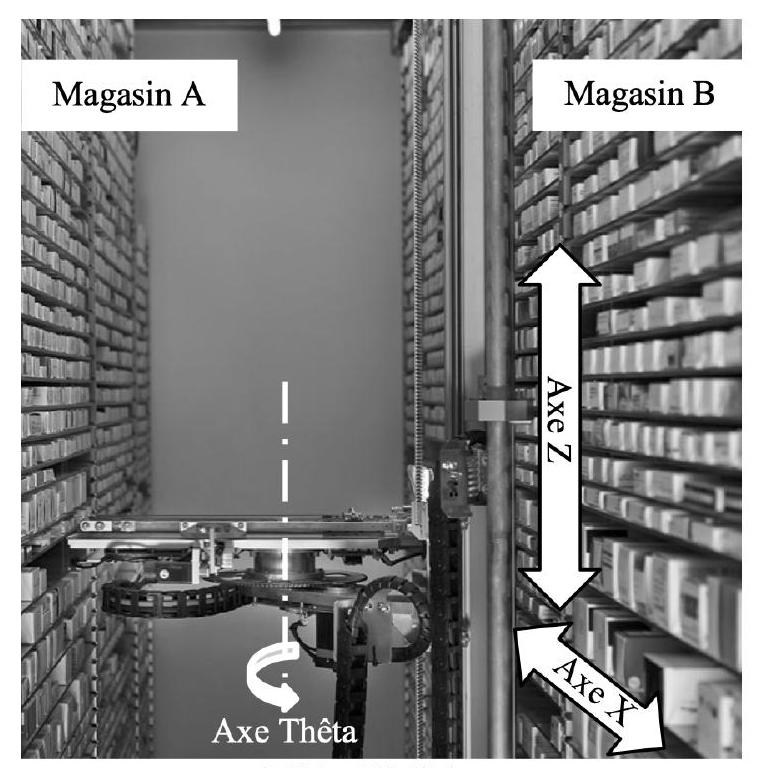
\includegraphics[height=5cm]{fig_01_a}
    \caption{Tête SLIM\label{fig:CCS_TSI_2021_fig_01_a}}
    \end{subfigure}
    \begin{subfigure}[b]{0.65\textwidth}
    \centering
    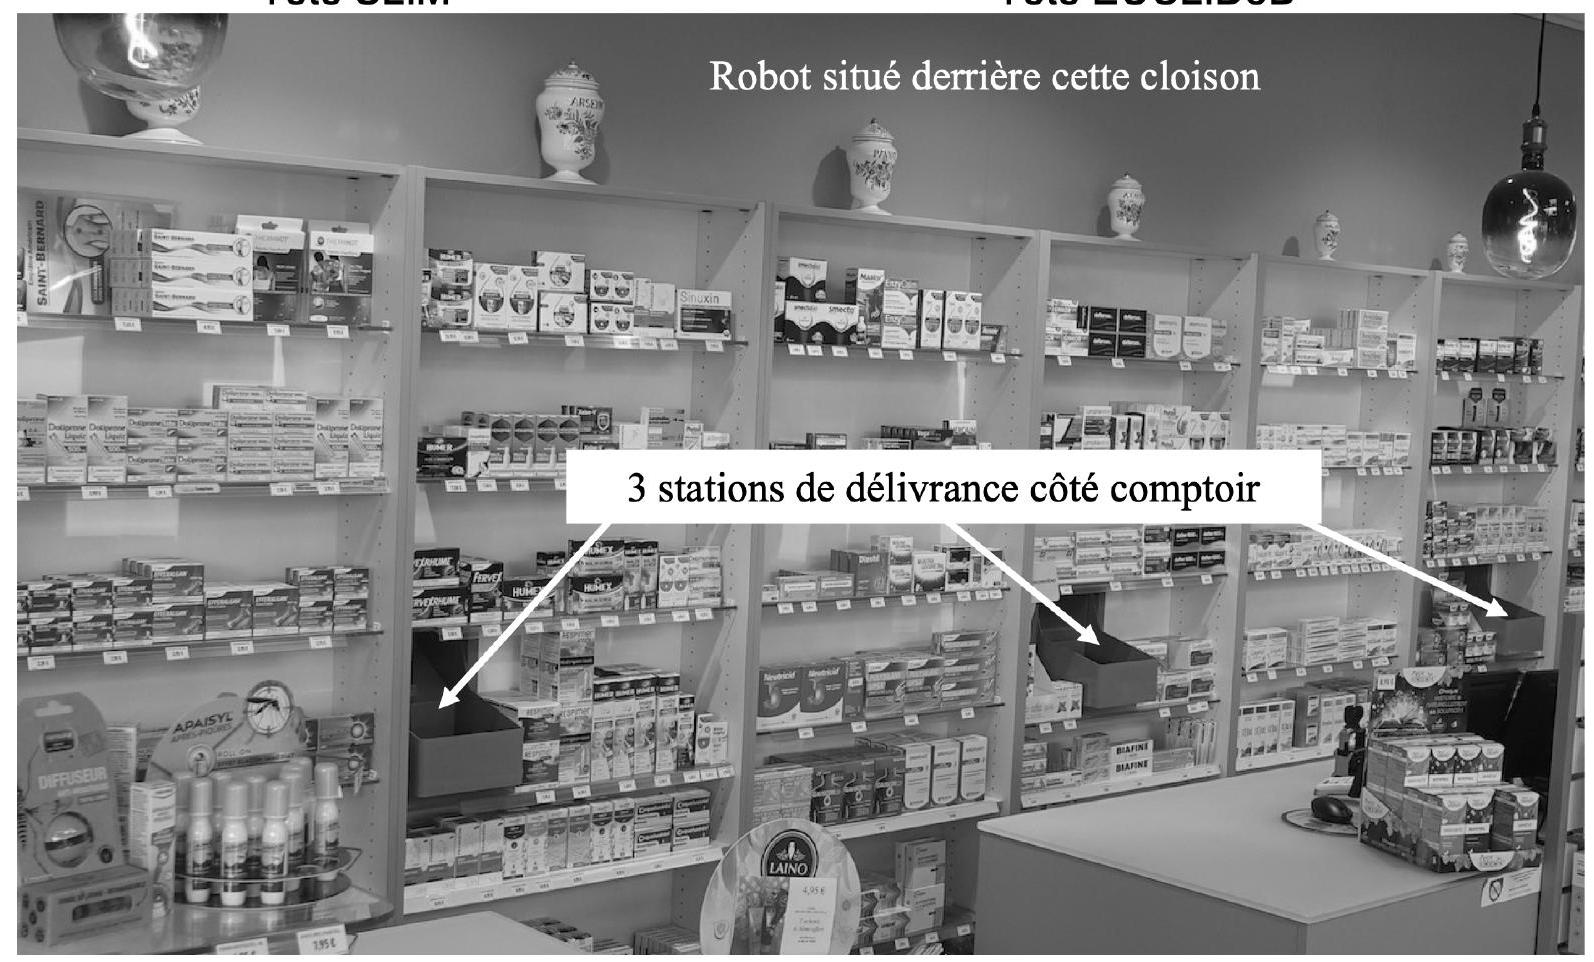
\includegraphics[height=5cm]{fig_01_b}
    \caption{Tête EUCLID3D\label{fig:image2}}
    \end{subfigure}

    \begin{subfigure}[b]{.9\textwidth}
    \centering
    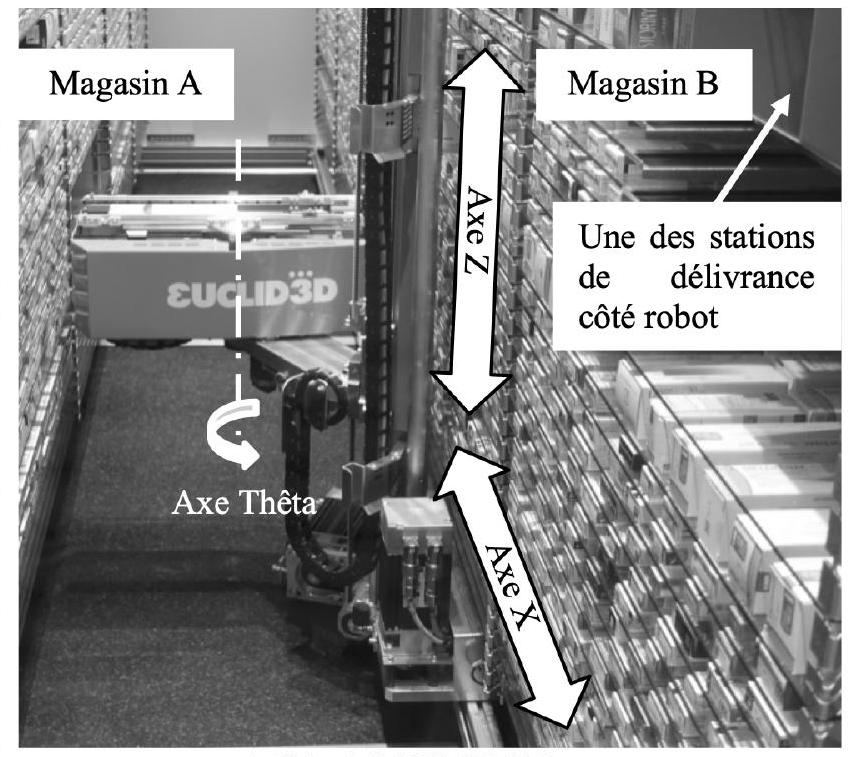
\includegraphics[width=\textwidth]{fig_01_c}
%    \caption{\label{fig:image3}}
    \end{subfigure}

\caption{Robot SINTESI avec un seul bras et sa tête SLIM ou sa tête EUCLID3D \label{fig:CCS_TSI_2021_fig_01}}%\subref{fig:image1} Picture 1, \subref{fig:image2} picture 2, \subref{fig:image3} picture 3, \subref{fig:image4} picture 4, \subref{fig:image5} picture 5.}
\end{figure}


Le robot SINTESI se présente sous la forme d'un couloir d'environ \SI{60}{cm} de large, bordé à gauche et à droite par deux magasins de stockage. Chaque magasin possède des étagères en verre de différentes hauteurs avec une profondeur utile de stockage d'environ \SI{35}{cm}. Le robot comporte ensuite un ou deux bras manipulateurs trois axes (ici un seul bras situé sur la droite de la photo), munis d'une tête de manipulation des boîtes dont deux versions sont proposées : la tête SLIM ou la tête EUCLID3D.

Le chargement des boîtes de médicaments dans le robot est hors du cadre de cette étude.

Ce sujet a pour but d'élaborer un modèle de simulation devant permettre d'apporter une aide décisionnelle sur le choix de la tête à implanter. Les résultats de simulation devront faire apparaître les écarts de performances du robot muni d'une tête simple (nommée SLIM) vis-à-vis d'une tête plus perfectionnée (nommée EUCLID3D).

Le robot SINTESI doit répondre aux exigences de la figure \ref{fig:CCS_TSI_2021_fig_02} qui seront validées tout au long du sujet.

\begin{figure}
\begin{center}
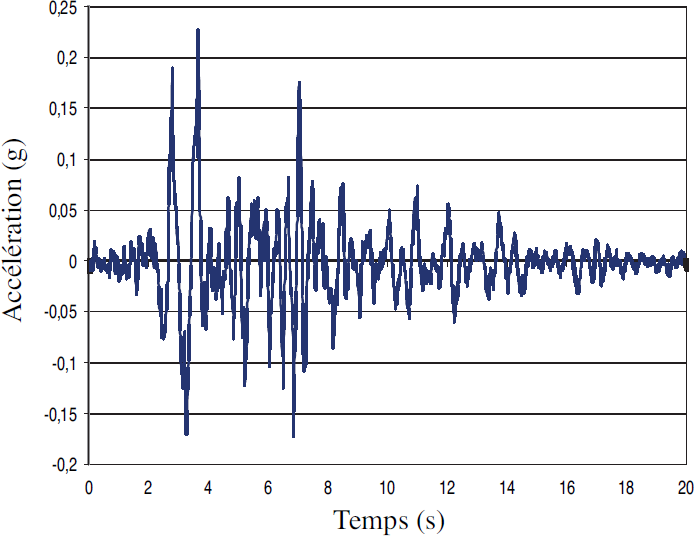
\includegraphics[max width=\textwidth]{fig_02}
\end{center}

\begin{center}
\begin{tabular}{|c|c|c|}
\hline
Exigence & Performance & Niveau \\
\hline
\multirow{8}{*}{Pilotage des axes} & \multirow[b]{2}{*}{Précisions des axes X et Z} & \begin{tabular}{l}
Erreur en régime permanent pour une consigne en \\
échelon inférieure à $0,5 \mathrm{~mm}$ \\
\end{tabular} \\
\hline
 &  & \begin{tabular}{l}
Erreur de traînage en régime permanent pour une \\
consigne en rampe (vitesse maximale) inférieure à \\
50 mm \\
\end{tabular} \\
\hline
 & \multirow{2}{*}{Stabilité des asservissements de position} & Marge de phase minimale de $45^{\circ}$ \\
\hline
 &  & Dépassement de l'axe Thêta inférieur à $1^{\circ}$ \\
\hline
 & Vitesses des axes X et Z & Vitesse maximale $v_{\max }=2,5 \mathrm{~m} \cdot \mathrm{s}^{-1}$ \\
\hline
 & Vitesse de l'axe Thêta & Vitesse maximale de $100^{\circ} \cdot \mathrm{s}^{-1}$ \\
\hline
 & Accélérations des axes X et Z & Accélération maximale de $a_{\max }=2 \mathrm{~m} \cdot \mathrm{s}^{-2}$ \\
\hline
 & Accélération de l'axe Thêta & Accélération maximale de $400^{\circ} \cdot \mathrm{s}^{-2}$ \\
\hline
\end{tabular}
\end{center}

\caption{\label{fig:CCS_TSI_2021_fig_02} Diagramme et tableau des exigences partielles du robot SINTESI}
\end{figure}

Certaines questions, peu ou pas guidées, demandent de l'initiative de la part du candidat. Leur énoncé est repéré par une barre en marge. Il est alors demandé d'expliciter clairement la démarche, les choix et de les illustrer, le cas échéant, par un schéma. Le barème valorise la prise d'initiative et tient compte du temps nécessaire à la résolution de ces questions.

%\section*{I Modélisation du robot SINTESI}
\section{Modélisation du robot SINTESI}
\begin{obj}
Analyser la structure du robot et établir des modèles comportementaux.
\end{obj}

%\section*{I.A - Architecture du bras manipulateur 3 axes}
\subsection{Architecture du bras manipulateur 3 axes}
\begin{obj}
Analyser la cinématique du bras manipulateur.
\end{obj}


Le bras manipulateur comprend trois axes: l'axe X , l'axe Z et l'axe Thêta dont la figure \ref{fig:CCS_TSI_2021_fig_03} et le tableau \ref{tab:CCS_TSI_2021_tab_01} précisent l'architecture.
\begin{figure}
\centering
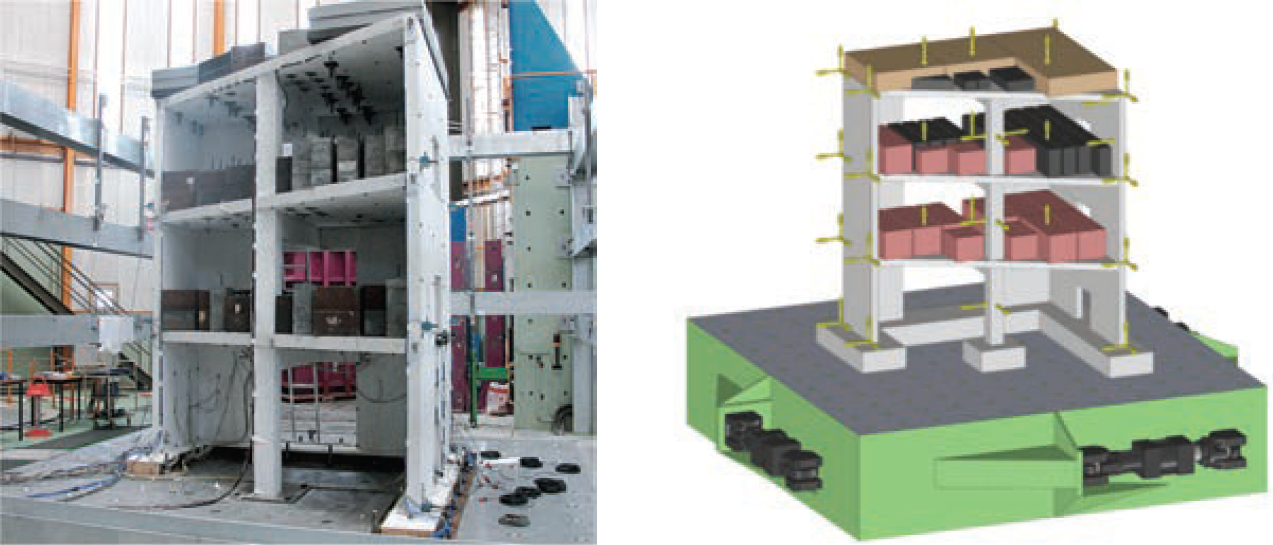
\includegraphics[max width=\textwidth]{fig_03}

\caption{\label{fig:CCS_TSI_2021_fig_03} Architecture du manipulateur 3 axes}
\end{figure}

\begin{table}
\centering
\begin{tabular}{|c|c|c|c|}
\hline
Axe & Axe X & Axe Z & Axe Thêta \\
\hline
Courses & de 0 à 10 m & de 0 à $2,5 \mathrm{~m}$ & de $\theta_{\min }$ à $\theta_{\max }$ \\
\hline
Pièces considérées & 10 par rapport à 0 & 20 par rapport à 10 & 30 par rapport à 20 \\
\hline
Mouvements & \begin{tabular}{c}
Translation \\
de direction $\vec{X}$ \\
\end{tabular} & \begin{tabular}{c}
Translation \\
de direction $\vec{Z}$ \\
\end{tabular} & \begin{tabular}{c}
Rotation \\
autour de l'axe $(F, \vec{Z})$ \\
\end{tabular} \\
\hline
Paramètres de position & $\overline{x(t)}$ & $\overline{z(t)}$ & $\overline{\theta(t)}$ \\
\hline
\end{tabular}

\caption{\label{tab:CCS_TSI_2021_tab_01}1 Paramétrage des mouvements des trois axes du robot}
\end{table}

Le schéma cinématique à compléter est fourni sur la figure \ref{fig:CCS_TSI_2021_fig_A} du document réponse.

%Q 1. 
\question{À l'aide du tableau \ref{tab:CCS_TSI_2021_tab_01}, proposer un graphe des liaisons d'une modélisation minimale restreinte aux solides $\mathbf{0}, \mathbf{1 0}, \mathbf{2 0}, \mathbf{3 0}$.}

%Q 2. 
\question{Compléter l'épure de la figure \ref{fig:CCS_TSI_2021_fig_A} du document réponse en représentant les liaisons correspondant au graphe des liaisons précédent.}

Le diagramme de définition de blocs du robot, dans la configuration étudiée (avec tête EUCLID3D), est donné à la figure \ref{fig:CCS_TSI_2021_fig_04}.

\begin{figure}
\centering
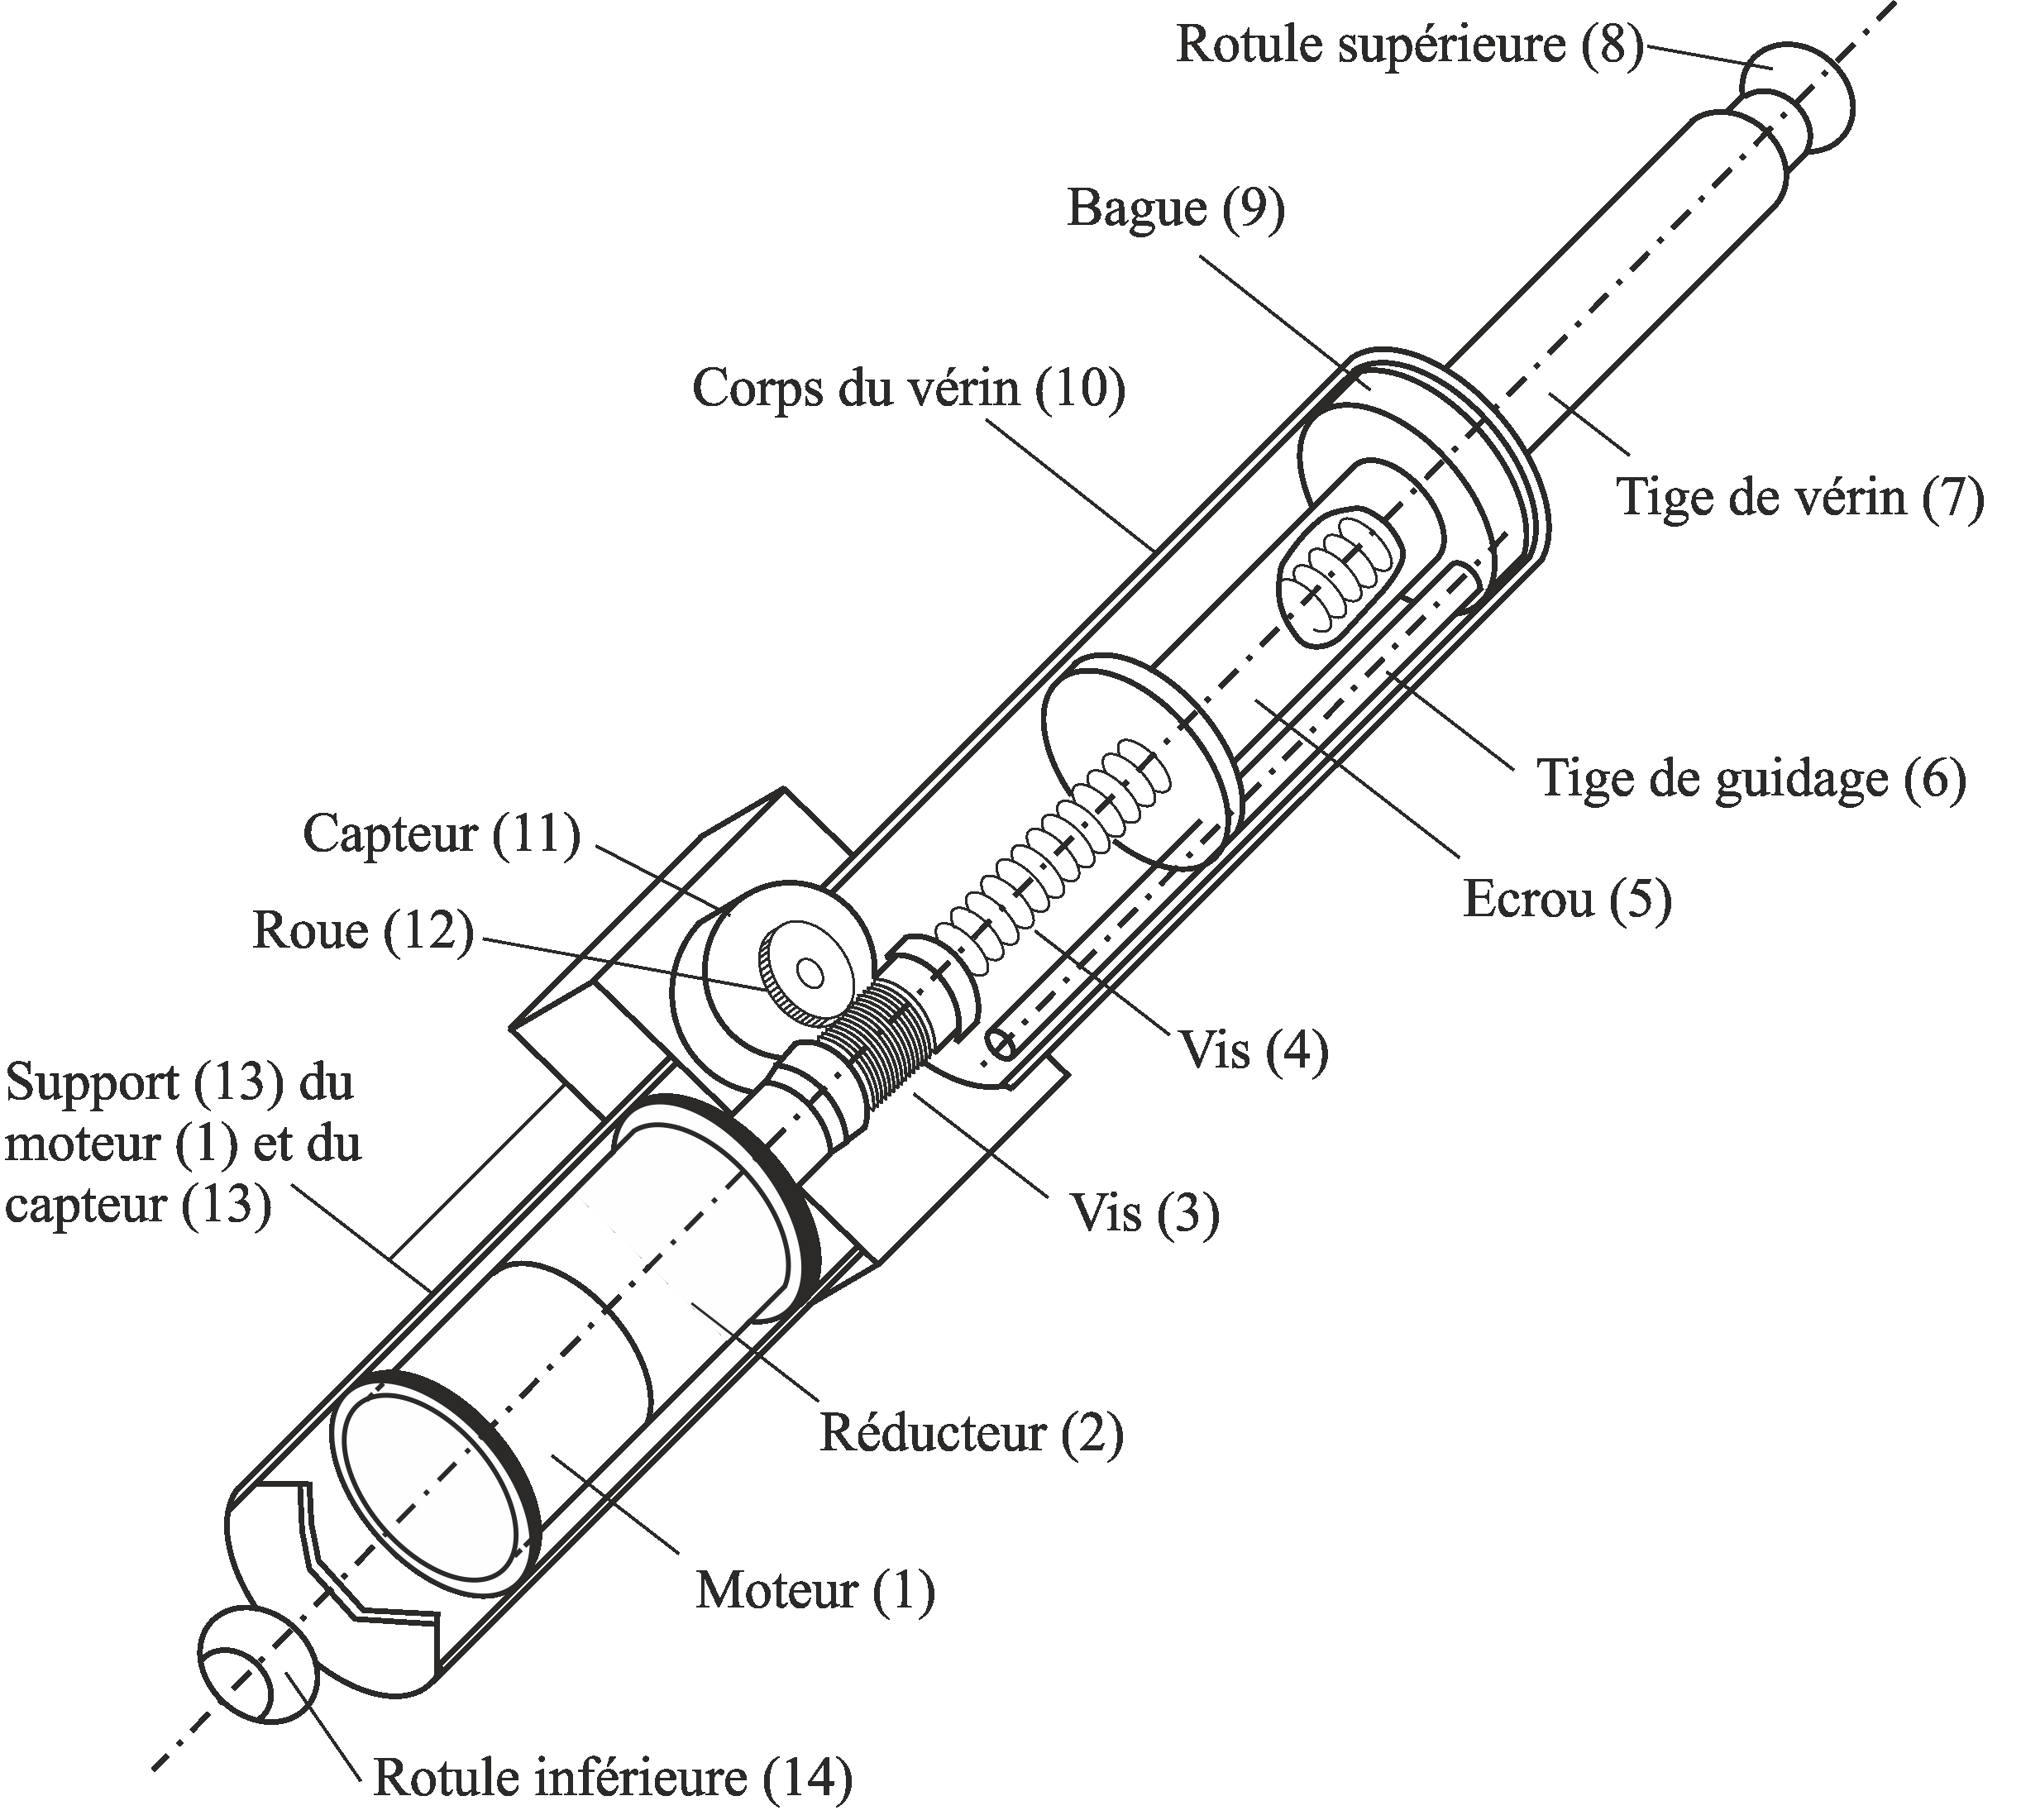
\includegraphics[max width=\textwidth]{fig_04}%2024_07_14_db927ae3a82093776e19g-04}

\caption{\label{fig:CCS_TSI_2021_fig_04}Diagramme de définition de blocs du robot SINTESI}
\end{figure}
Le paramétrage est fourni dans le tableau \ref{tab:CCS_TSI_2021_tab_02}.

%Q 3. 
\question{À l'aide du paramétrage et des valeurs figurant dans le tableau \ref{tab:CCS_TSI_2021_tab_02} et sur la figure \ref{fig:CCS_TSI_2021_fig_A} du document réponse, déterminer les expressions littérales et les valeurs numériques des paramètres $\rho_{1}$ et $\rho_{x}$ tels que $\omega_{12}(t)=\rho_{1} \omega_{11}(t)$ et $v_{x}(t)=\rho_{x} \omega_{11}(t)$ en précisant l'unité de $\rho_{x}$.}

\begin{table}
\centering
A REMPACERR....
\begin{tabular}{|c|c|c|c|c|}
\hline
Solide & Nom & Repère associé & \begin{tabular}{c}
Paramétrage \\
des mouvements \\
\end{tabular} & \begin{tabular}{c}
Masse et grandeurs \\
cinétiques \\
\end{tabular} \\
\hline
0 & Bâti & $(O, \vec{X}, \vec{Y}, \vec{Z})$ &  &  \\
\hline
10 & Chariot & $(A, \vec{X}, \vec{Y}, \vec{Z})$ & \begin{tabular}{c}
$\overrightarrow{O A}=x(t) \vec{X}$ \\
$\vec{V}_{10 / 0}(A)=v_{x}(t) \vec{X}$ \\
$\vec{a}_{10 / 0}(A)=a_{x}(t) \vec{X}$ \\
$v_{x}(t)=\rho_{x} \omega_{11}(t)$ \\
\end{tabular} & \begin{tabular}{c}
$m_{10}=20 \mathrm{~kg}$ \\
\hline
12 \\
\hline
\end{tabular} \\
\hline
\end{tabular}

\caption{\label{tab:CCS_TSI_2021_tab_02}Paramétrage dimensionnel et cinétique}
\end{table}

%\section*{I.B - Analyse des déplacements mesurés}
\subsection{Analyse des déplacements mesurés}
\begin{obj}
Analyser la stratégie de pilotage des axes du robot.
\end{obj}

Une campagne de mesures, à l'aide d'un accéléromètre (nommé module AHRS - Attitude and Heading Reference System - sur la figure \ref{fig:CCS_TSI_2021_fig_05}) placé sur la tête EUCLID3D, a été effectuée.

Le fichier de points récupéré est un fichier au format csv. Après traitement sous Python, les trois tableaux Numpy ci-dessous à une dimension sont créés :

\begin{itemize}
  \item temps : vecteur des temps avec une période d'échantillonnage constante $T_{e}=0,01 \mathrm{~s}$, temps $[i]$ est donc égal à $i T_{e}$;

  \item $\boldsymbol{a x}$ : vecteur des accélérations selon $\vec{X}, a x[i]$ est donc la valeur de l'accélération selon $\vec{X}$ à l'instant $i T_{e}$;

  \item $\boldsymbol{a} \boldsymbol{z}$ : vecteur des accélérations selon $\vec{Z}$ (l'accélération de la pesanteur $\vec{g}$, qui est également mesurée par l'accéléromètre, est xxxxxxxxx

\end{itemize}

\begin{figure}
\centering
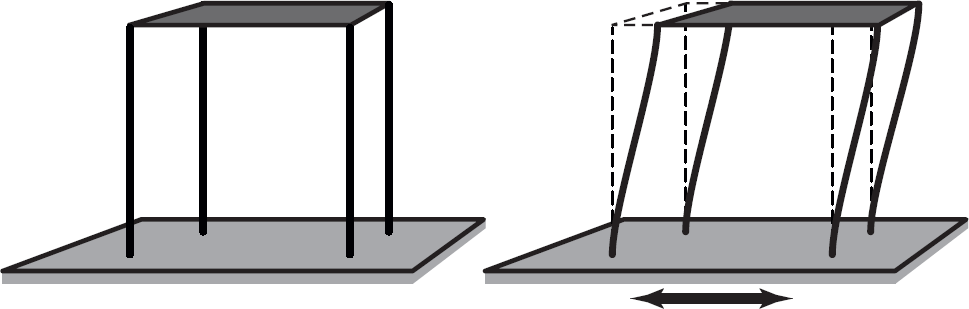
\includegraphics[max width=.5\textwidth, center]{fig_05}
\caption{\label{fig:CCS_TSI_2021_fig_05}Implantation du module AHRS sur la tête EUCLID3D supposée compensée et donc n'est pas à prendre en compte).}
\end{figure}

Le tracé des accélérations brutes permet d'obtenir le graphe de la figure \ref{fig:CCS_TSI_2021_fig_06} .

L'exploitation des mesures nécessite la mise en place d'un filtrage afin d'accéder aux accélérations moyennes du bras. Un filtre passe-bas du premier ordre, de gain unitaire et de constante de temps tau $=5 \cdot T_{e}$ est appliqué aux vecteurs $a \boldsymbol{x}$ et $\boldsymbol{a} \boldsymbol{z}$ pour donner respectivement les vecteurs $a x f$ et $\boldsymbol{a} \boldsymbol{z f}$.

%Q 4. 
\question{Donner l'équation différentielle temporelle qui lie les grandeurs $a_{x}(t)$ et $a_{x f}(t)$ puis l'équation de récurrence associée sur les vecteurs $\boldsymbol{a x}$ et $\boldsymbol{a} \boldsymbol{z}$ à l'aide d'un schéma de dérivation numérique à gauche ou arrière. Le résultat sera présenté sous la forme $a x f[i]=A \cdot a x f[i-1]+B \cdot a x[i]$ où les constantes $A$ et $B$ seront exprimées en fonction de $T_{e}$ et de tau. Les variables $T_{e}$ et tau sont des variables globales.}


\begin{figure}
\centering
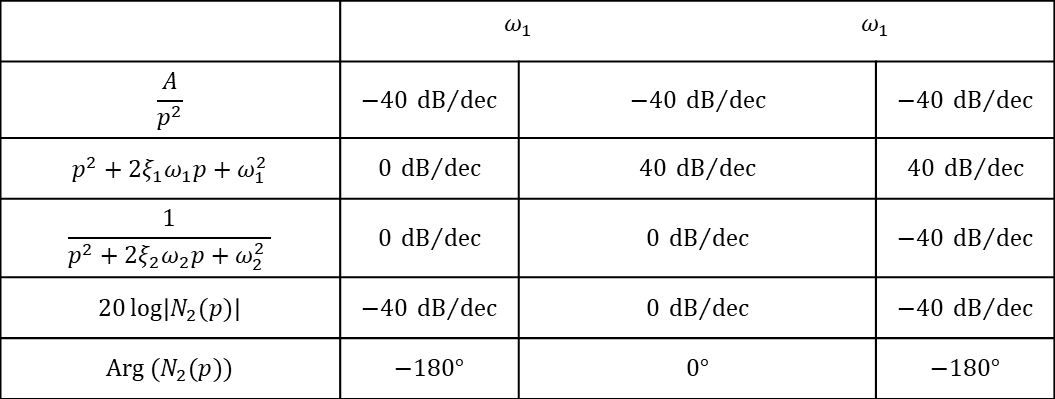
\includegraphics[max width=.5\textwidth]{fig_06}%{2024_07_14_db927ae3a82093776e19g-06}
\caption{\label{fig:CCS_TSI_2021_fig_06}Graphes des accélérations brutes sous Python}
\end{figure}

Le début du script permettant de définir le vecteur $\boldsymbol{a x f}$ est donné ci-dessous :

\begin{verbatim}
import numpy as np
#Filtrage
N=ax.shape[0]
axf=np.zeros(N)
axf[0]= ax[0]
\end{verbatim}

%Q 5.
\question{Compléter le script précédent pour définir le vecteur $\boldsymbol{a x f}$, correspondant au résultat du filtre passe-bas du premier ordre sur le vecteur connu $a x$.}

%Q 6. 
\question{En utilisant la méthode des rectangles et la variable $N$, écrire un script permettant de définir le vecteur $\boldsymbol{v} \boldsymbol{x} \boldsymbol{f}$ des vitesses filtrées selon $\vec{X}$ à partir du vecteur $\boldsymbol{a} \boldsymbol{x} \boldsymbol{f}$.}

À l'aide d'une nouvelle intégration, puis en appliquant aussi ces scripts selon $\vec{Z}$, les tracés de la figure \ref{fig:CCS_TSI_2021_fig_07} sont obtenus.

\begin{figure}
\centering
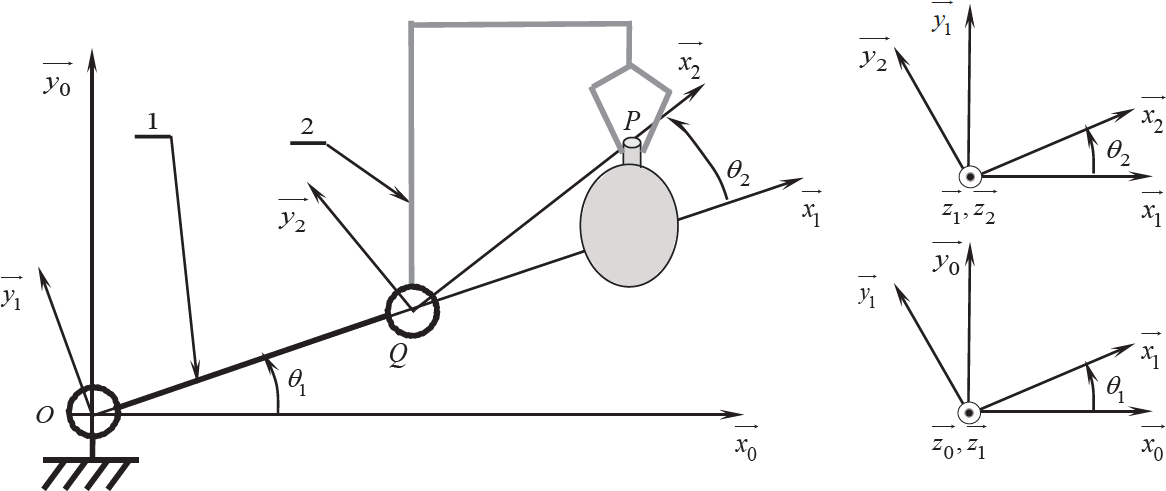
\includegraphics[max width=\textwidth]{fig_07}%{2024_07_14_db927ae3a82093776e19g-06(1)}
\caption{\label{fig:CCS_TSI_2021_fig_07}Graphes des grandeurs cinématiques filtrées sous Python}
\end{figure}

%Q 7. 
\question{À l'aide de la figure \ref{fig:CCS_TSI_2021_fig_07}, estimer les valeurs maximales des accélérations et des vitesses mesurées selon $\vec{X}$. Analyser les différences entre les résultats de mesures et les spécifications figurant dans le tableau des exigences figure~\ref{fig:CCS_TSI_2021_fig_02} .}

Dans ce cas particulier, c'est l'axe X qui impose le temps de déplacement complet puisque l'amplitude du déplacement selon $\vec{X}$ est supérieure à celle selon $\vec{Z}$. Dans la suite du sujet, la vérification du dimensionnement de la motorisation se fera uniquement sur l'axe $X$.

Renseigner les paramètres de modèles comportementaux du bras en translation selon $\vec{X}$.

Le profil de pilotage utilisé par le constructeur suit un profil en trapèze des vitesses. Dans le cas de l'amplitude de déplacement étudiée de $2,7 \mathrm{~m}$, ce profil se simplifie en un triangle des vitesses symétrique (voir figure \ref{fig:CCS_TSI_2021_fig_08}) puisque la vitesse maximale ne peut pas être obtenue pendant le déplacement limité de $2,7 \mathrm{~m}$.

Les valeurs des accélérations utilisées sont les accélérations maximales spécifiées dans le tableau des exigences. On considère l'origine des temps au début du mouvement.

%Q 8. 
\question{Tracer les allures des évolutions temporelles de l'accélération $a_{x}(t)$ et du déplacement $x(t)$ en précisant les valeurs caractéristiques en fonction de $t_{1}, t_{2}$ et $v_{1}$.}

\begin{figure}
\centering
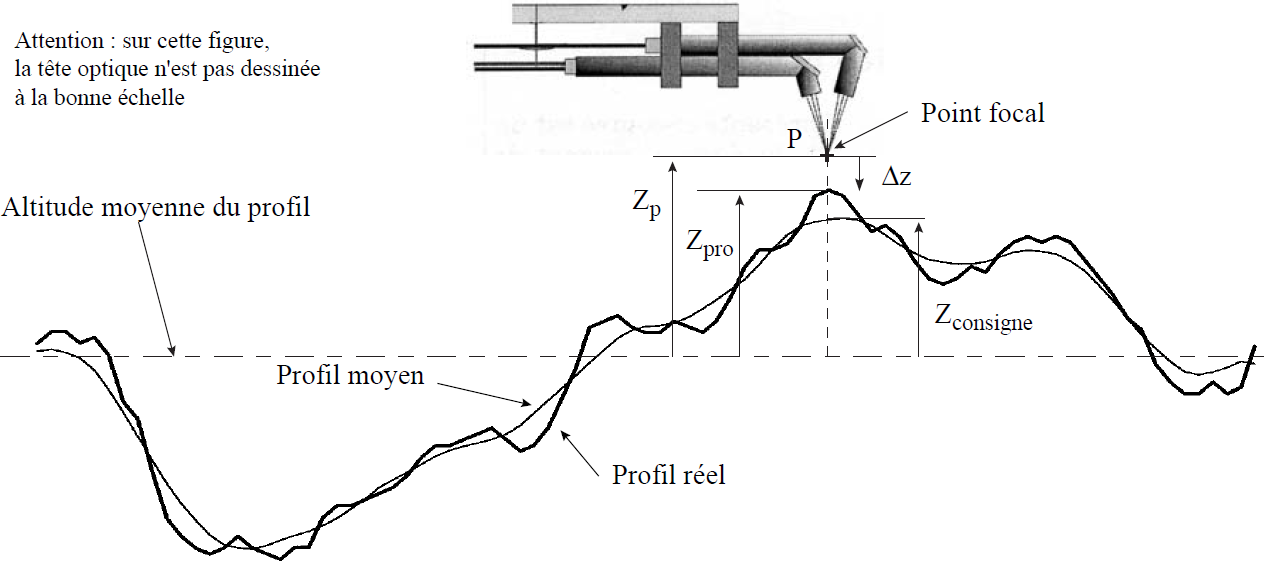
\includegraphics[max width=.5\textwidth]{fig_08}%{2024_07_14_db927ae3a82093776e19g-07}
\caption{\label{fig:CCS_TSI_2021_fig_08} Profil simplifié des vitesses utilisé}
\end{figure}


%Q 9. 
\question{Après avoir déterminé $v_{1}$ en fonction de $a_{\max }$ et $t_{1}$, déterminer le temps de mouvement $t_{2}$ permettant d'effectuer $2,7 \mathrm{~m}$ selon $\vec{X}$ avec ce profil des vitesses.}

La motorisation est réalisée au moyen de l'association d'une machine synchrone triphasée et d'un variateur dont la structure est fournie à la figure \ref{fig:CCS_TSI_2021_fig_09}.


\begin{figure}
\centering
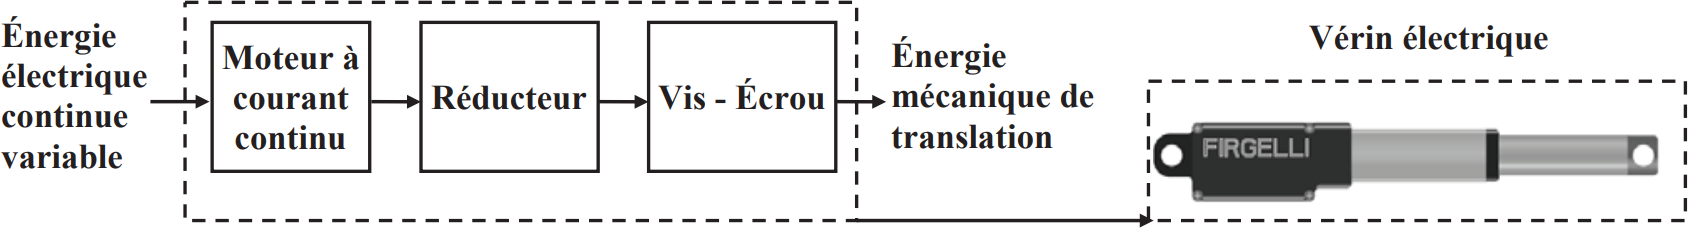
\includegraphics[max width=\textwidth]{fig_09}%{2024_07_14_db927ae3a82093776e19g-07(1)}

\caption{\label{fig:CCS_TSI_2021_fig_09}Schéma générique de l'association d'un variateur et d'une machine} synchrone
\end{figure}

Les caractéristiques de la machine sont données dans le tableau \ref{tab:CCS_TSI_2021_tab_03}.

\begin{table}
\centering
\begin{tabular}{|c|c|c|c|}
\hline
\multicolumn{4}{|c|}{Moteur} \\
\hline
Grandeur & Valeur & Grandeur & Valeur  \\
\hline
Couplage des enroulements & étoile & Nombre de pôles & 6  \\
\hline
Tension nominale entre phases & 210 V & Constante de f.e.m phase/phase & $0,54 \mathrm{~V} \cdot \mathrm{s} \cdot \mathrm{rad}^{-1}$  \\
\hline
Couple rotor bloqué & $3,28 \mathrm{~N} \cdot \mathrm{m}$ & Résistance phase/phase & $5,96 \Omega$   \\
\hline
Couple à vitesse nominale & $3,93 \mathrm{~N} \cdot \mathrm{m}$ & Inductance phase $/$ phase & $19,3 \mathrm{mH}$   \\
\hline
Puissance à vitesse nominale & 1235 W & Intensité de pointe & $9,49 \mathrm{~A}$ \\
\hline
Vitesse nominale & $3000 \mathrm{tr} \cdot \mathrm{min}^{-1}$ & Intensité nominale & $4,2 \mathrm{~A}$ \\
\hline
Couple impulsionnel & $8,86 \mathrm{~N} \cdot \mathrm{m}$ &  &   \\
\hline
\multicolumn{4}{|c|}{Codeur incrémental} \\
\hline
\multicolumn{2}{|c|}{2500 points par tour} &  \multicolumn{2}{|c|}{2 voies}  \\
\hline
\end{tabular}

\caption{\label{tab:CCS_TSI_2021_tab_03}Caractéristiques du moteur HDT B10S}
\end{table}

Le schéma équivalent, de la machine synchrone, pour une phase, ainsi que le diagramme de Fresnel correspondant sont rappelés à la figure \ref{fig:CCS_TSI_2021_fig_10}.\\

\begin{figure}
\centering
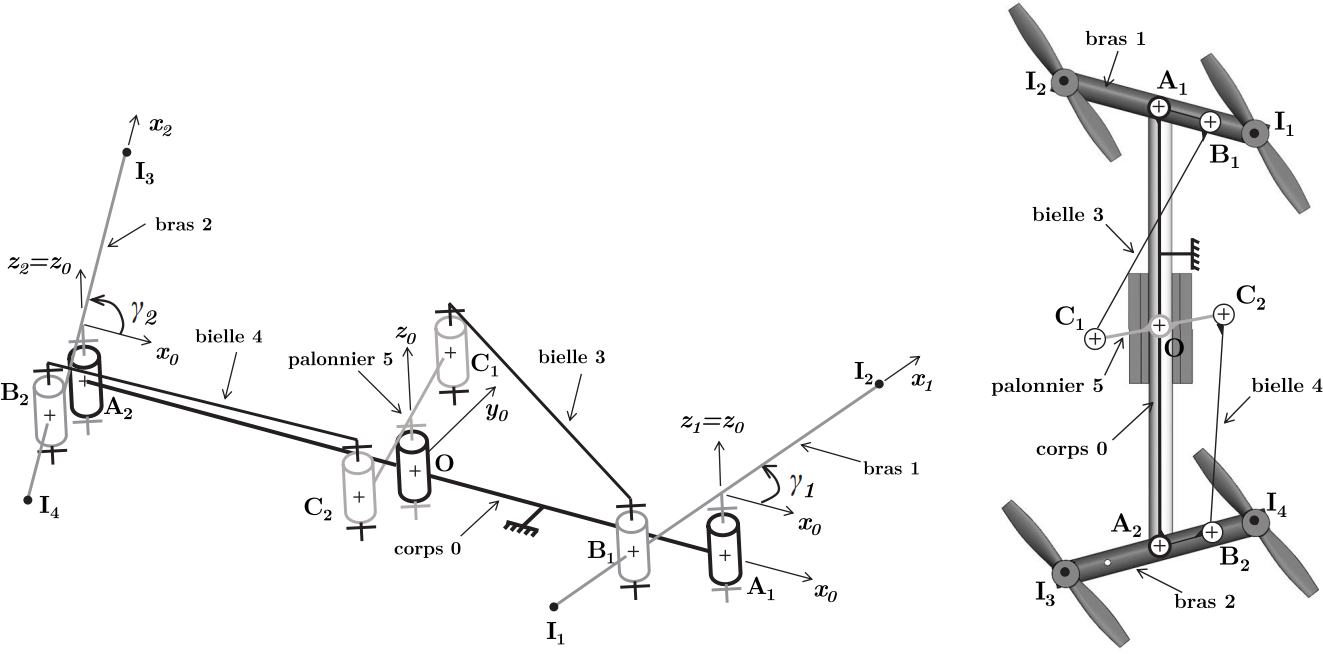
\includegraphics[max width=\textwidth, center]{fig_10}
\caption{\label{fig:CCS_TSI_2021_fig_10}Schéma équivalent d'un enroulement de la machine synchrone}
\end{figure}

Les outils de simulation mettant en œuvre des machines synchrones autopilotées demandent souvent des temps de calcul importants. Ceux-ci peuvent être considérablement réduits en utilisant un modèle simplifié.

Le but du questionnement qui suit est d'élaborer le modèle d'une machine à courant continu équivalente afin de simuler le comportement du robot suite à une consigne de prise de boîte de médicaments. Dans le modèle équivalent, seules les pertes dans le cuivre seront prises en compte.

%Q 10. 
\question{Donner l'expression de la loi des mailles liant les variables $\underline{V}, \underline{E}, \underline{I_{s}}$ et les paramètres $R$ et $L$.}

%Q 11. 
\question{Donner l'expression de la puissance électromagnétique $P_{e m}$ développée par la machine synchrone en fonction des variables $E, I_{s}$ et $\psi$.}

L'autopilotage assuré par le variateur permet de fixer l'angle $\psi$ à $0^{\circ}$ ou $180^{\circ}$ suivant le mode de fonctionnement de la machine.

%Q 12.
\question{Montrer que, dans ce cas, l'expression du couple électromagnétique $C_{e m}$ est de la même forme que pour une machine à courant continu. Déterminer la valeur de la constante de couple $K$ en précisant l'unité.}

Par la suite on prendra $K=0,9 \mathrm{~Wb}$. Le modèle équivalent pour la simulation est donné figure \ref{fig:CCS_TSI_2021_fig_11}.



\begin{figure}
\centering
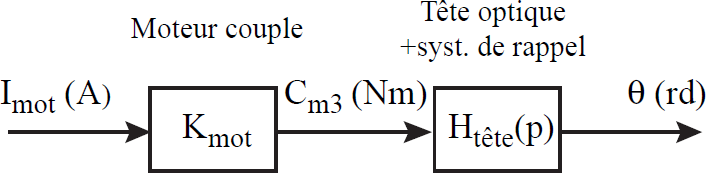
\includegraphics[max width=.5\textwidth]{fig_11}%{2024_07_14_db927ae3a82093776e19g-08}
\caption{\label{fig:CCS_TSI_2021_fig_11}Modèle de la machine à courant continu équivalente.}
\end{figure}


Ce modèle doit permettre d'obtenir le point nominal en régime permanent compte tenu que seules les pertes dans le cuivre sont prises en compte.

%Q 13. 
\question{Déterminer la valeur du courant nominal de la machine à courant continu équivalente permettant d'obtenir le même couple nominal que la machine synchrone.}

%Q 14. 
\question{Calculer la valeur de la résistance d'induit r permettant d'obtenir les mêmes pertes joules que la machine synchrone.}

Par la suite on prendra une valeur de $r=8 \Omega$.

%Q 15. 
\question{Déterminer la valeur de la tension $U_{N}$ de la machine à courant continu équivalente afin d'obtenir le point de fonctionnement nominal.}

%\section*{I.D - Validation du dimensionnement de l'axe $\boldsymbol{X}$}
\subsection{Validation du dimensionnement de l'axe $\boldsymbol{X}$}
\begin{obj}
Valider le choix de la motorisation de l'axe X.
\end{obj}


Dans la suite du sujet, un modèle causal simplifié ou un modèle acausal seront utilisés suivant les parties d'étude et les performances à valider. Ces deux types de modélisation, pour le moteur seul, sont rappelés à la figure \ref{fig:CCS_TSI_2021_fig_12}, $J$ étant l'inertie du rotor du moteur.


\begin{figure}
\centering
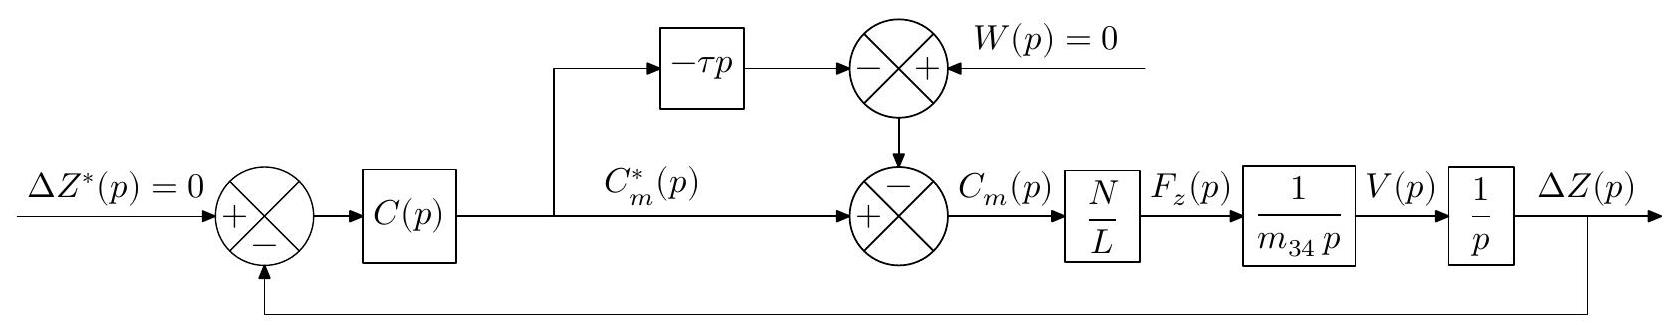
\includegraphics[max width=\textwidth]{fig_12}%{2024_07_14_db927ae3a82093776e19g-09}
\caption{\label{fig:CCS_TSI_2021_fig_12}Modèles causal et modèle acausal de la MCC équivalente.}
\end{figure}




Une simulation à vide $\left(C_{r}=0\right)$ du moteur de l'axe X a été réalisée. Les deux modèles ont été renseignés de façon à obtenir le même comportement dynamique que la machine réelle. La réponse à un échelon de tension de 320 V a donné les résultats de la figure \ref{fig:CCS_TSI_2021_fig_13}.


\begin{figure}
\centering
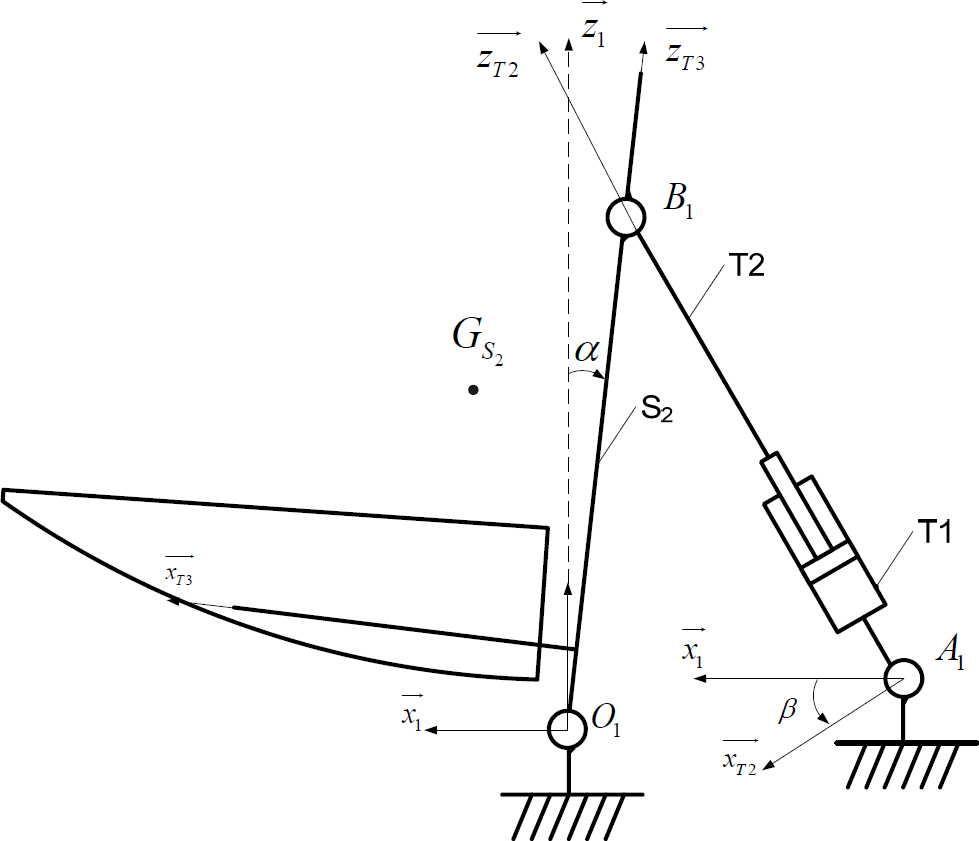
\includegraphics[max width=\textwidth]{fig_13}%{2024_07_14_db927ae3a82093776e19g-09(1)}
\caption{\label{fig:CCS_TSI_2021_fig_13}Réponses à un échelon et zoom de l'évolution de vitesse.}
\end{figure}

%Q 16. 
\question{Justifier l'ordre de grandeur de la valeur numérique du courant de démarrage du moteur.}

%Q 17. 
\question{À partir du modèle causal proposé à la figure \ref{fig:CCS_TSI_2021_fig_12}, déterminer l'expression de $\left.\frac{\Omega_{m}(p)}{U(p)}\right|_{C_{r}=0}$ sous forme canonique.}

%Q 18. 
\question{À partir de la figure \ref{fig:CCS_TSI_2021_fig_13}, retrouver la valeur de l'inertie $J$ qui a été renseignée dans les modèles et comparer cette valeur à celle du constructeur qui figure dans le tableau \ref{tab:CCS_TSI_2021_tab_02}.}

Seul le mouvement de l'axe X est étudié dans cette partie. Ainsi, $\vec{\Omega}_{13 / 10}=\overrightarrow{0}, \vec{\Omega}_{30 / 20}=\overrightarrow{0}$ et $\vec{\Omega}_{31 / 20}=\overrightarrow{0}$.

%Q 19. 
\question{Exprimer littéralement l'énergie cinétique galiléenne de l'ensemble E des pièces en mouvement par rapport au référentiel galiléen 0 sous la forme $E_{c}(E / 0)=\frac{1}{2} J_{1 e q} \omega_{11}(t)^{2}$ où $J_{1 e q}$ sera exprimée en fonction des masses et inerties qui apparaissent dans le tableau \ref{tab:CCS_TSI_2021_tab_02} ainsi que des paramètres $\rho_{1}$ et $\rho_{x}$.}

Indépendamment des résultats précédents, les valeurs $J_{1 e q}=8 \times 10^{-3} \mathrm{~kg} \cdot \mathrm{m}^{2}$ et $\rho_{x}=0,01 \mathrm{~m}$ sont retenues pour la suite.

Les pertes dans les transmissions sont supposées négligeables ainsi que les efforts résistants. La puissance intérieure à l'ensemble E se limite donc à la puissance délivrée par le moteur.

%Q 20. 
\question{Déterminer alors le couple $C_{m}$ nécessaire à fournir par le moteur de l'axe X pour l'accélération maximale du diagramme des exigences et comparer cette valeur à celle fournie dans le tableau 3\ref{tab:CCS_TSI_2021_tab_03}.}

Les paramètres du modèle de simulation de l'axe X sont maintenant connus. La même démarche peut être effectuée pour l'axe Z dont la motorisation est similaire à celle de l'axe X.

%\section*{II Validation des performances du robot}
\section{Validation des performances du robot}
\begin{obj}
Valider les choix du constructeur par rapport aux performances attendues.
\end{obj}

%\section*{II.A - Justification et dimensionnement des résistances de dissipation}
\subsection{Justification et dimensionnement des résistances de dissipation}
\begin{obj}
Vérifier la nécessité des résistances de dissipation et les dimensionner.
\end{obj}

Le modèle acausal correspondant au déplacement aller et retour du robot selon $\vec{X}$ est présenté à la figure \ref{fig:CCS_TSI_2021_fig_14}.


\begin{figure}
\centering
   \begin{subfigure}[b]{.9\textwidth}
    \centering
    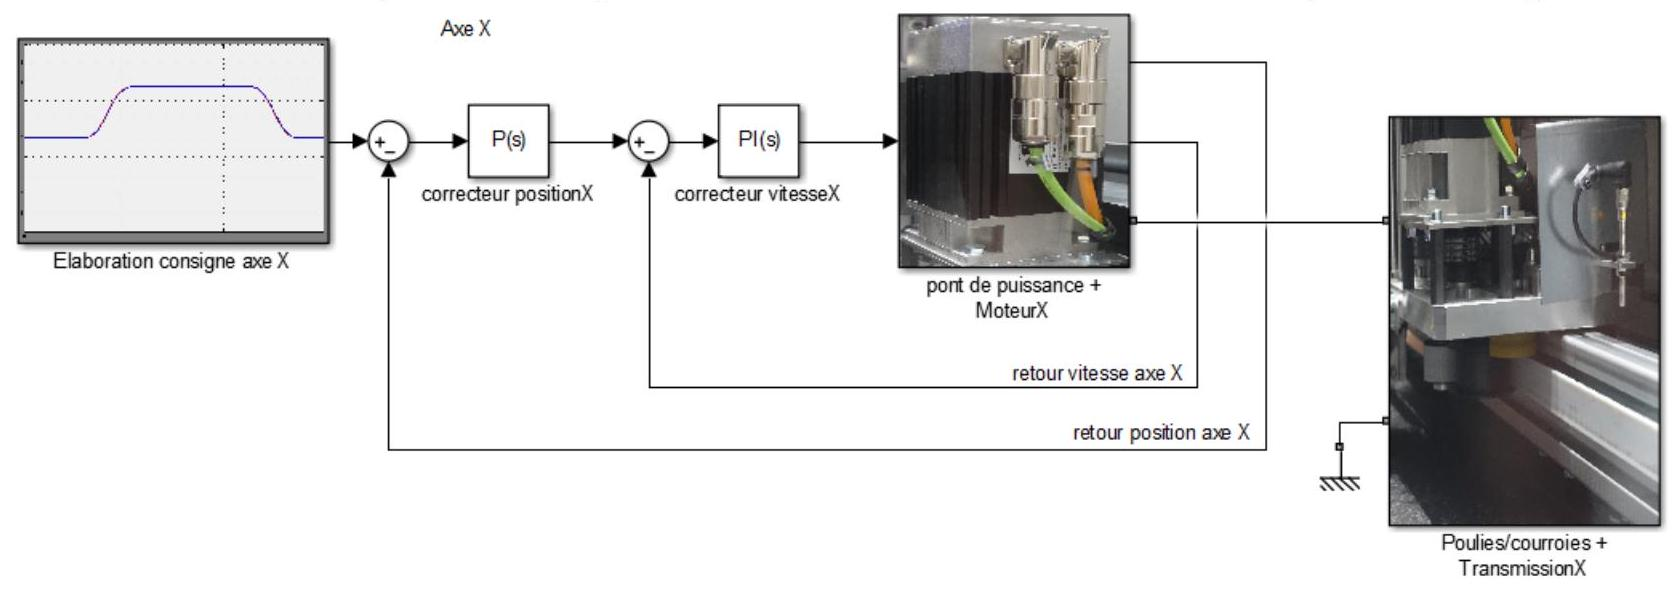
\includegraphics[width=\textwidth]{fig_14_a}
      \end{subfigure}
    
    \begin{subfigure}[b]{0.45\textwidth}
    \centering
    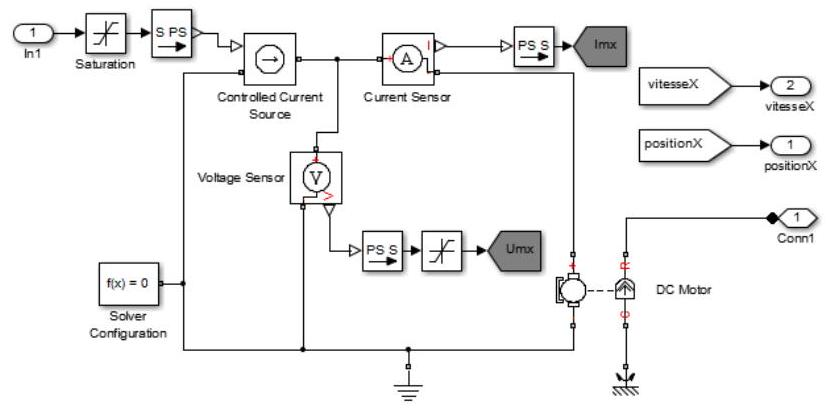
\includegraphics[width=\textwidth]{fig_14_b}
    \caption{Pont de puissance + moteur axe X \label{fig:CCS_TSI_2021_fig_14_b}}
    \end{subfigure}
    \begin{subfigure}[b]{0.45\textwidth}
    \centering
    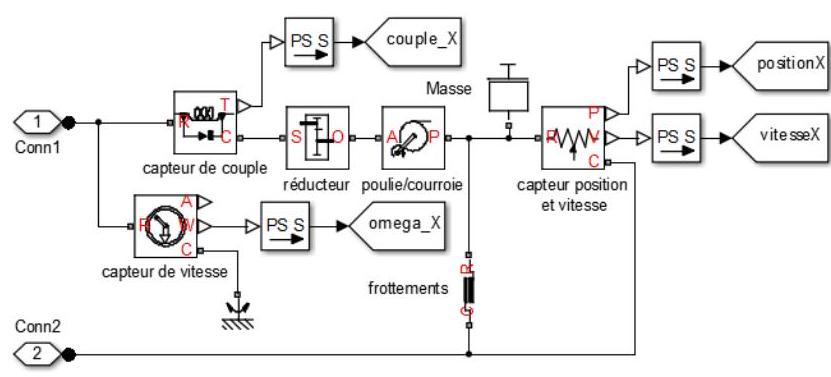
\includegraphics[width=\textwidth]{fig_14_c}
    \caption{Poulies/courroie et transmission axe X
\label{fig:CCS_TSI_2021_fig_14_c}}
    \end{subfigure}

\caption{\label{fig:CCS_TSI_2021_fig_14}Modèle de simulation de l'axe $X$.}
\end{figure}


Les résultats de simulation sont présentés à la figure \ref{fig:CCS_TSI_2021_fig_15}.
\begin{figure}
\centering
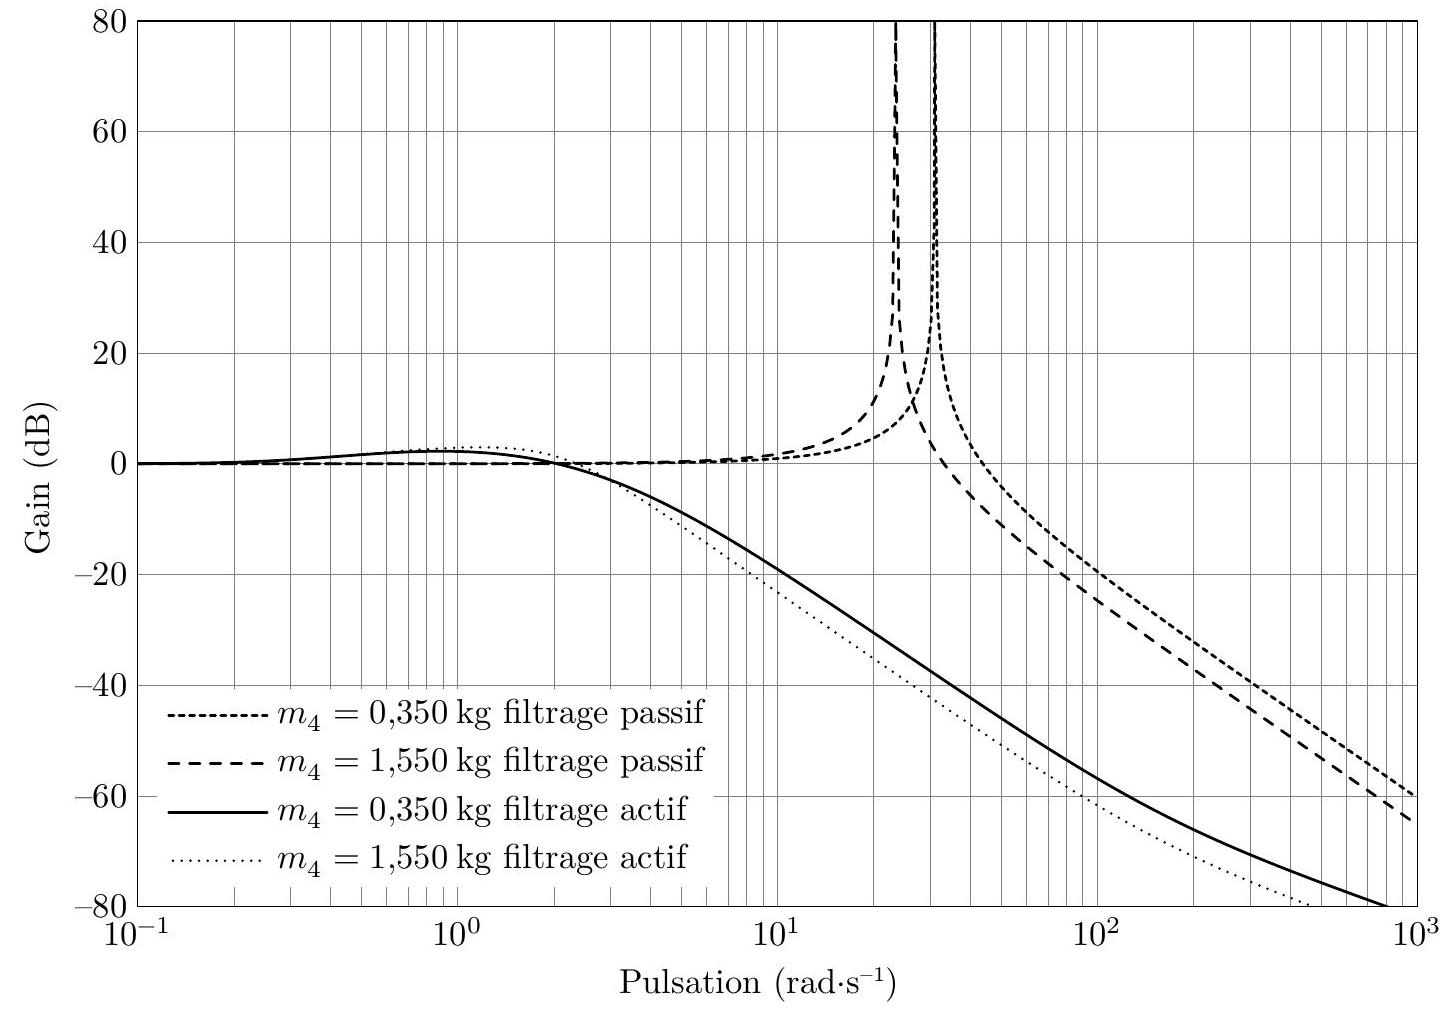
\includegraphics[max width=\textwidth]{fig_15}
\caption{\label{fig:CCS_TSI_2021_fig_15}Résultats de simulation pour un déplacement aller/retour selon $\vec{X}$ de $2,7 \mathrm{~m}$.}
\end{figure}
Ces résultats temporels ont été reproduits sur la figure \ref{fig:CCS_TSI_2021_fig_B} du document réponse avec une approximation de l'évolution temporelle du couple moteur.

%Q 21. 
\question{En assimilant le couple à sa valeur approchée, tracer sur la figure \ref{fig:CCS_TSI_2021_fig_B} du document réponse, l'allure de la puissance délivrée par le moteur. Déduire de ce relevé la nécessité d'un module de dissipation au niveau des variateurs des machines synchrones (figure \ref{fig:CCS_TSI_2021_fig_09}).}

%Q 22. 
\question{En considérant que le cycle précédant se reproduise en permanence, estimer la puissance crête et la puissance moyenne que doit présenter la résistance de dissipation. Le constructeur du variateur préconise une résistance de $39 \Omega$ (référence R90W39R) de puissance nominale 90 W et de puissance crête de 3 kW . Valider la référence préconisée.}

%\section*{II.B - Réglage des asservissements de position}
\subsection{Réglage des asservissements de position}

\begin{obj}
Régler les correcteurs des variateurs afin de valider les performances de positionnement.
\end{obj}

Le robot pharmathek réalise des déplacements suivant les axes X et Z en fonction des consignes de position issues d'un logiciel spécifique de traitement d'ordonnances. En fonction des boites demandées, celui-ci recherche dans sa base l'emplacement des différentes boites et envoie aux variateurs les consignes de déplacement. Le bon fonctionnement du système dépend du réglage du correcteur de position en termes de stabilité et de suivi de consigne.

L'étude qui suit se limite au dimensionnement du correcteur de l'axe X. Bien que le traitement soit numérique, la période de traitement sera considérée très petite par rapport aux constantes de temps du système afin de traiter le problème avec les outils des systèmes linéaires continus et invariants.

La structure globale de la boucle de position (documentation constructeur) est donnée à la figure \ref{fig:CCS_TSI_2021_fig_16}.

\begin{figure}
\centering
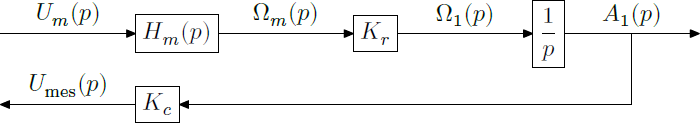
\includegraphics[max width=\textwidth]{fig_16}
\caption{\label{fig:CCS_TSI_2021_fig_16}Structure de la boucle de position du variateur donnée par le constructeur.}
\end{figure}
%Q 23. 

\question{Identifier les différentes boucles présentes dans la structure de la figure \ref{fig:CCS_TSI_2021_fig_16}. Déterminer sur quelle grandeur mécanique agit le bloc de limitation de courant.}

Les variateurs ont la possibilité d'être pilotés par un logiciel dédié. Deux essais, limités à la boucle de vitesse, avec des consignes en échelon de 300 et $1200 \mathrm{tr} \cdot \mathrm{min}^{-1}$ ont été réalisés afin d'établir un modèle simplifié de l'asservissement de vitesse. Les résultats des essais sont donnés à la figure \ref{fig:CCS_TSI_2021_fig_17}.

\begin{figure}
\centering
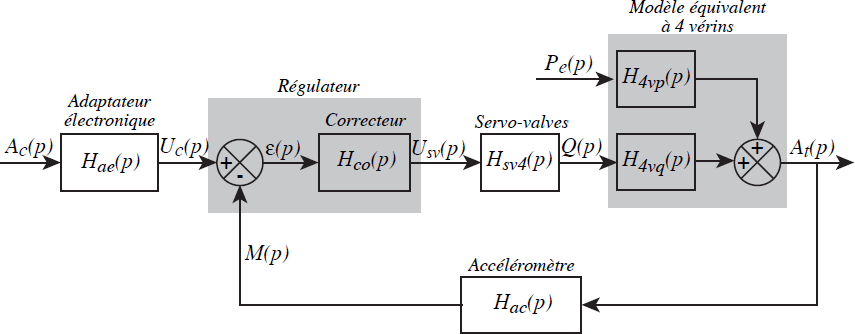
\includegraphics[max width=\textwidth]{fig_17}
\caption{\label{fig:CCS_TSI_2021_fig_17}Résultats des essais à un échelon de vitesse}
\end{figure}

%Q 24. 
\question{Justifier le fait que les deux relevés ne présentent pas la même allure. Préciser le nom de l'élément du schéma bloc de la figure \ref{fig:CCS_TSI_2021_fig_16} qui intervient.}

%Q 25. 
\question{Identifier les paramètres $K$ et $\tau$ du modèle du premier ordre de la boucle de vitesse tels que }

$$
H(p)=\frac{\Omega_{m}(p)}{\Omega_{c}(p)}=\frac{K}{1+\tau p}
$$

Pour l'étude du correcteur de position, l'asservissement de position non perturbé peut se modéliser par le schéma bloc donné à la figure \ref{fig:CCS_TSI_2021_fig_18} dans lequel la boucle de vitesse est remplacée par sa fonction de transfert $H(p)$.

\begin{figure}
\centering
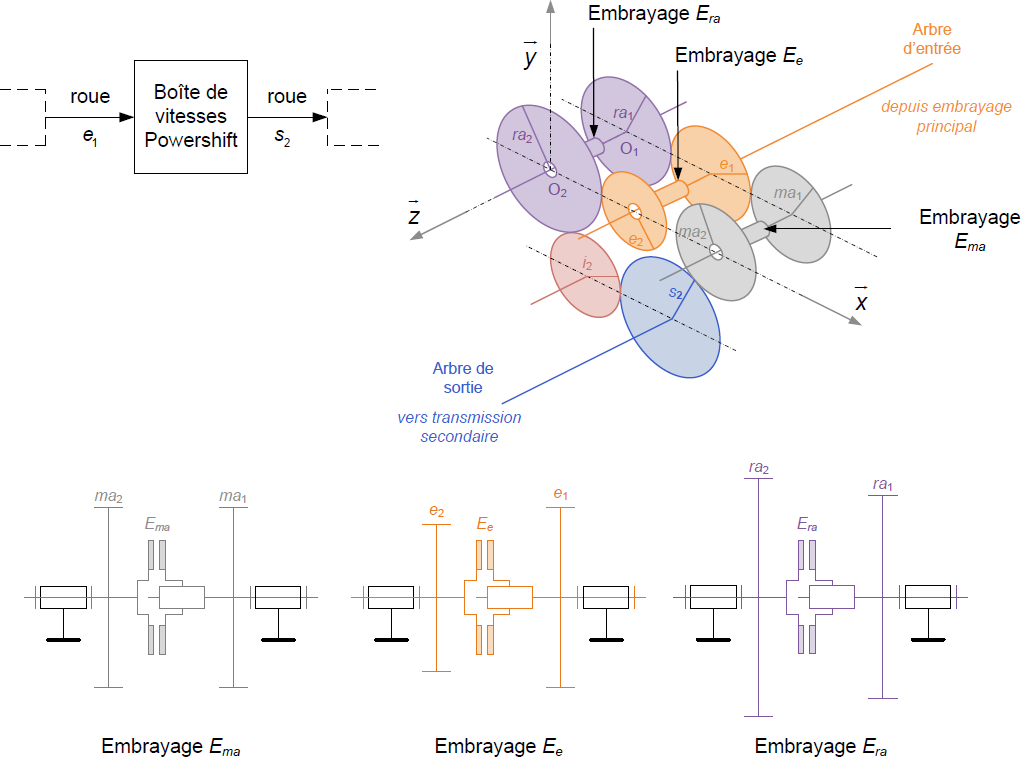
\includegraphics[max width=\textwidth]{fig_18}
\caption{\label{fig:CCS_TSI_2021_fig_18}Schéma bloc de la boucle de position $\left(\omega_{m}(t)=\omega_{11}(t)\right)$.}
\end{figure}


Le codeur, de type incrémental (voir tableau \ref{tab:CCS_TSI_2021_tab_02}), placé sur l'arbre moteur, délivre 2500 points par tour sur 2 voies soit 10000 points par tour.

%Q 26. 
\question{Déterminer la valeur de $K_{\text {cod }}$ en points $\cdot \operatorname{rad}^{-1}$ puis celle de l'adaptateur de consigne $A$ en points $\cdot \mathrm{m}^{-1}$.}

%Q 27. 
\question{Déterminer la résolution du codeur incrémental et vérifier qu'elle est compatible avec les exigences de précision du tableau des exigences (figure \ref{fig:CCS_TSI_2021_fig_02}).}

Le correcteur $C(p)$ est un correcteur proportionnel de valeur $K_{p}$. La fonction de transfert $H(p)$ sera prise égale à $H(p)=\frac{1}{1+\tau p}$ avec $\tau=20 \mathrm{~ms}$.

%Q 28. 
\question{Déterminer l'expression littérale de la fonction de transfert en boucle ouverte $\operatorname{FTBO}(p)$.}

Le diagramme de Bode de la fonction de transfert en boucle ouverte $F T B O(j \omega)$ lorsque $K_{p}=1$ est donné sur la figure \ref{fig:CCS_TSI_2021_fig_C} du document réponse.

%Q 29. 
\question{Déterminer la valeur de $K_{p}$ permettant de satisfaire à l'exigence de marge de phase.}

Les variateurs des axes X et Z reçoivent les consignes de déplacement du logiciel de traitement des ordonnances. La loi d'évolution de la consigne est alors élaborée par le variateur en fonction du profil de vitesse défini figure \ref{fig:CCS_TSI_2021_fig_08}.

Le but du questionnement à venir est de vérifier si le système est capable de suivre une consigne de position de type «rampe », lorsque la vitesse est constante. Le schéma bloc de la figure \ref{fig:CCS_TSI_2021_fig_18} peut se réduire à celui de la figure \ref{fig:CCS_TSI_2021_fig_19} avec $K_{1}=70$ après réglage de $K_{p}$.

\begin{figure}
\centering
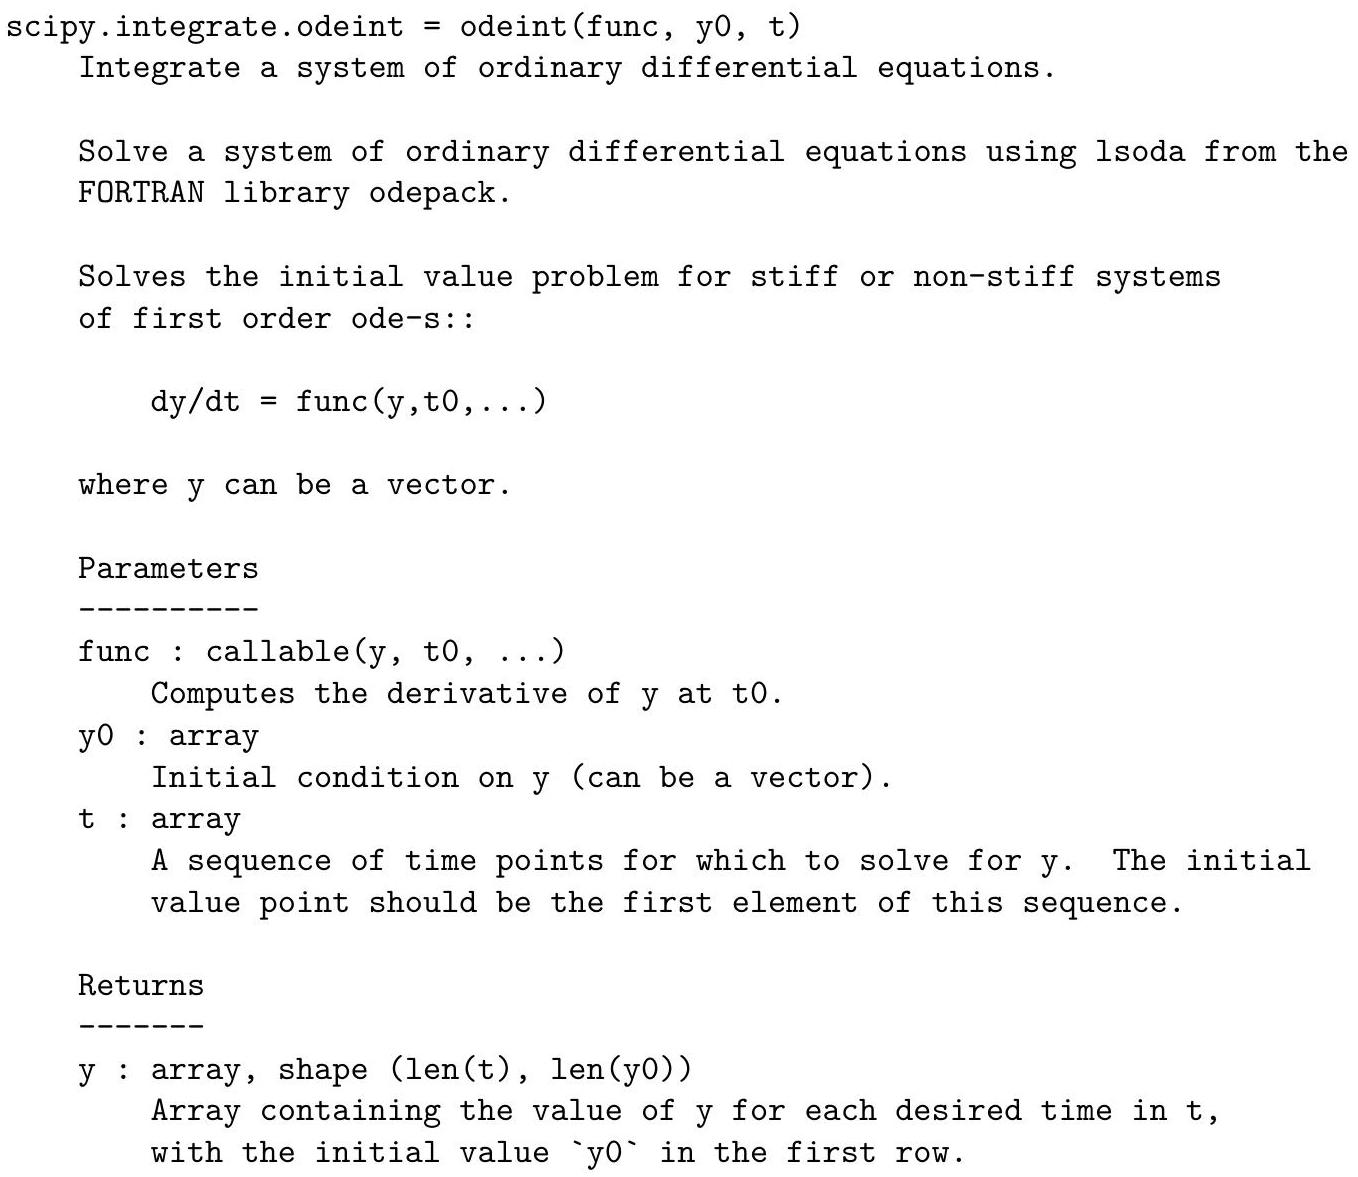
\includegraphics[max width=\textwidth]{fig_19}

\caption{\label{fig:CCS_TSI_2021_fig_19}Schéma bloc équivalent.}
\end{figure}


%Q 30. 
\question{Déterminer l'erreur en régime permanent (erreur de traînage) $\Delta x_{v}=\lim _{t \rightarrow \infty} \mu(t)$ en fonction de $K_{1}$ lorsque l'entrée de consigne de position est une rampe de pente $V_{x}$ constante. Il est rappelé la transformée de Laplace :}

$$
x_{c}(t)=V_{x} t \stackrel{\mathcal{L}}{\rightarrow} X_{c}(p)=\frac{V_{x}}{p^{2}}
$$

%Q 31. 
\question{Conclure sur la capacité du système à suivre les lois d'évolution des consignes de position en translation vis-à-vis des exigences du tableau de la figure \ref{fig:CCS_TSI_2021_fig_02}.}

%Objectif
\begin{obj}
Valider l'intérêt de l'option tête EUCLID3D par rapport à la tête SLIM dans le cadre de la problématique d'optimisation du temps de délivrance d'une ordonnance et de l'énergie consommée.
\end{obj}

\subsubsection{Présentation du système de préhension}
La tête EUCLID3D, comme la tête SLIM (voir figure \ref{fig:CCS_TSI_2021_fig_20}), saisit les boîtes de médicaments grâce à une pince constituée de deux mors en fibres de carbone qui peuvent s'écarter (mouvement d'ouverture et de serrage) et translater (mouvement d'entrée et de sortie de la pince).

La pince (voir figure \ref{fig:CCS_TSI_2021_fig_21}) permet alors de faire glisser les boîtes de l'étagère de stockage sur le tablier de la tête ou inversement. Lors de la saisie, l'écartement des deux mors est affecté à la valeur de la largeur $l i$ de la boîte $i$.

\begin{figure}
\centering
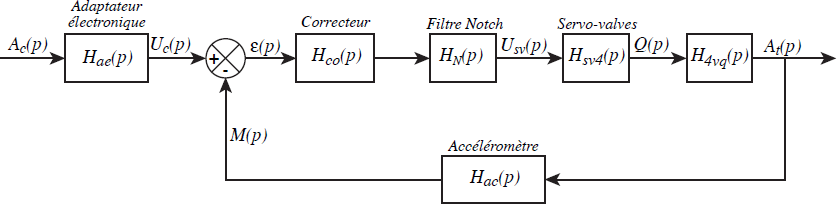
\includegraphics[max width=.3\textwidth]{fig_20}

\caption{\label{fig:CCS_TSI_2021_fig_20}Photo de la tête SLIM}
\end{figure}



\begin{figure}
\centering
xxxxxx
mouvement d'entrée et de sortie de la pince
xxxx
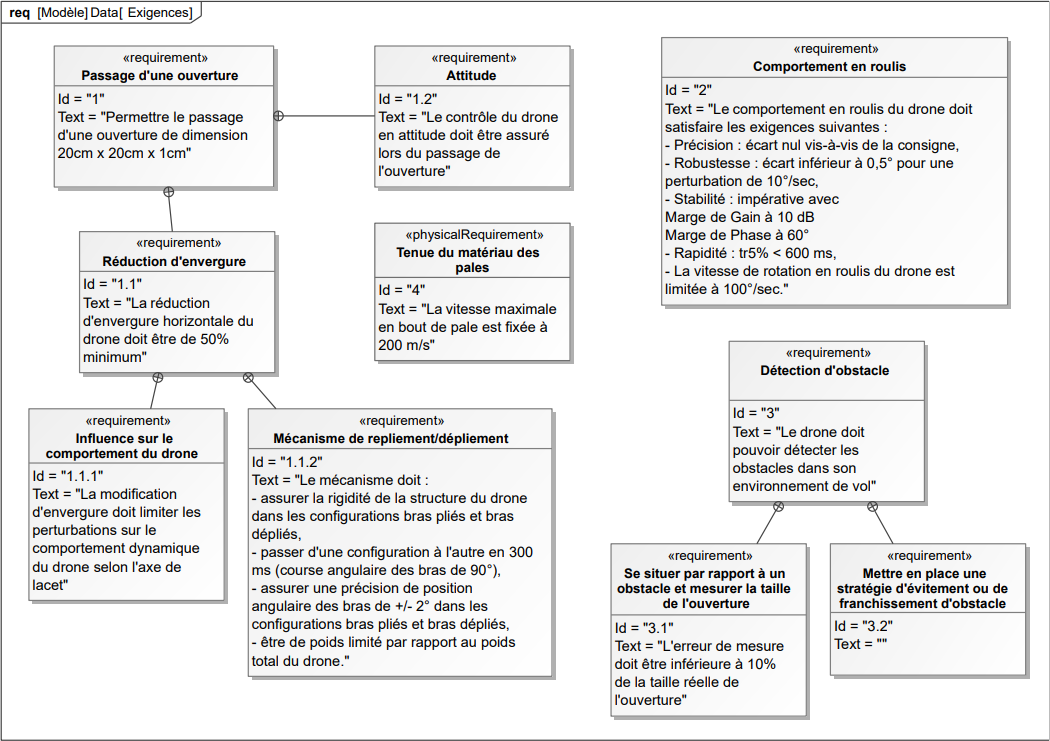
\includegraphics[max width=\textwidth]{fig_21}
\caption{\label{fig:CCS_TSI_2021_fig_21}Vue de dessus de la pince.}
\end{figure}

%\section*{II.C.2) Validation du gain de temps}
\subsubsection{Validation du gain de temps}

La tête EUCLID3D (voir figure \ref{fig:CCS_TSI_2021_fig_23}) se distingue de la tête SLIM grâce à un stockage temporaire des médicaments sous le tablier qui peut s'ouvrir. La tête SLIM n'étant pas munie de ce système de stockage temporaire, ne dispose pas de système de manœuvre du tablier, ni de tapis roulant ni de trappe permettant l'évacuation des boîtes de la zone de stockage.

Les boîtes sont toutes stockées de la même façon sur les étagères des magasins, posées sur leur plus grande face. Elles sont placées avec des largeurs croissantes dans le sens de la profondeur de l'étagère. La figure \ref{fig:CCS_TSI_2021_fig_22} est une photo de l'écran de contrôle donnant la disposition d'une des étagères du magasin B. Le tableau \ref{tab:CCS_TSI_2021_tab_04} fournit la description des symboles utilisés dans le graphe d'états de la figure \ref{fig:CCS_TSI_2021_fig_D} du document réponse.

\begin{figure}
\centering
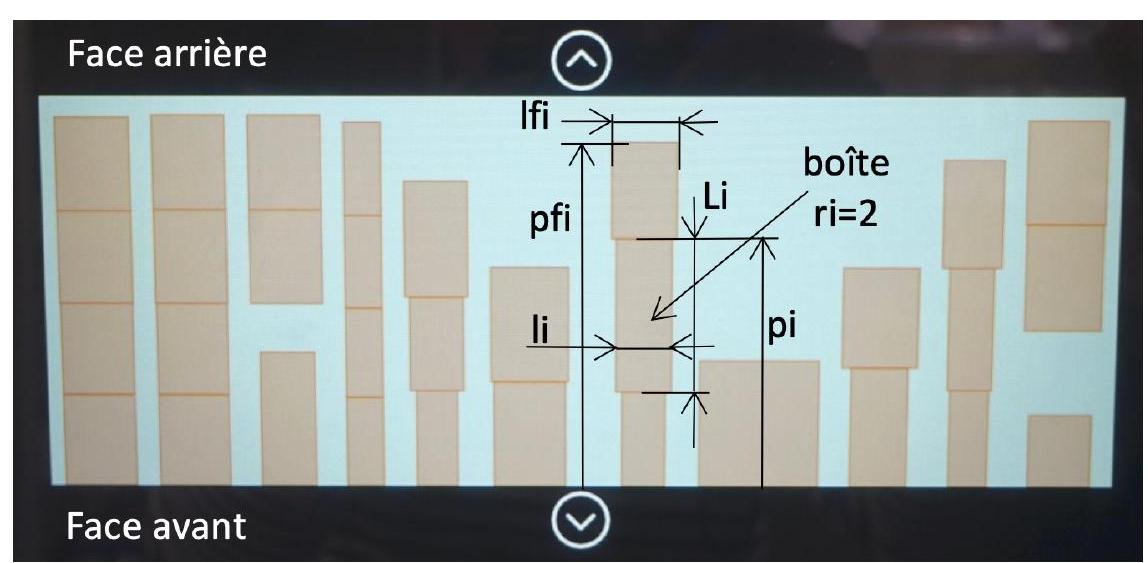
\includegraphics[max width=\textwidth, center]{fig_22}\\
\caption{\label{fig:CCS_TSI_2021_fig_22}Vue de la disposition sur une étagère.}
\end{figure}



\begin{table}
\centering
\begin{tabular}{|c|c|}
\hline
Variables globales ou internes & Commentaires \\
\hline
position & Position de la tête $(\mathrm{X}, \mathrm{Y})$ \\
\hline
délivrance & Position de la zone de délivrance \\
\hline
i & Indice \\
\hline
n & Nombre de références (boîtes) de l'ordonnance (ici $\mathrm{n}=3$ ) \\
\hline
posi & Position de la boîte i \\
\hline
li & Longueur de la boîte i boîte i \\
\hline
Li & Profondeur de la boîte i \\
\hline
pi & Largeur de la boîte du fond sur la rangée i \\
\hline
ri & Profondeur de la boîte du fond sur la rangée i \\
\hline
lfi &  \\
\hline
pfi &  \\
\hline
\end{tabular}

\caption{\label{tab:CCS_TSI_2021_tab_04} Symboles utilisés}
\end{table}

Le trajet étudié consiste à délivrer une ordonnance composée de trois références successives situées en trois positions différentes (pos1, pos2 et pos3) conformément au tableau \ref{tab:CCS_TSI_2021_tab_05}.

\begin{table}
\centering
\begin{tabular}{|l|c|c|c|c|}
\hline
 & délivrance & pos1 & pos2 & pos3 \\
\hline
Position selon X (en mètres) & 0 & 2 & 1 & -2 \\
\hline
Rang de la boîte ri &  & $\mathrm{r} 1=2$ & $\mathrm{r} 2=1$ & $\mathrm{r} 3=1$ \\
\hline
\end{tabular}

\caption{\label{tab:CCS_TSI_2021_tab_05}Informations pour les trois positions relatives successives par rapport à la position de délivrance.}
\end{table}

Entre deux déplacements, la tête doit saisir la boîte correspondant à la référence sur la rangée, puis la traiter. Compte tenu de l'étendue des déplacements, c'est le mouvement de l'axe X qui impose la durée de déplacement.

À l'instant initial :

\begin{itemize}
  \item le bras manipulateur est à la position de délivrance d'une ordonnance ;

  \item les pinces sont écartées et rentrées ;

  \item le tablier est fermé ;

  \item la tige de poussée est rentrée ;

  \item la trappe est fermée et le tapis roulant arrêté.

\end{itemize}

La tête SLIM retourne à la position de délivrance après la prise de chaque boîte de médicaments, ce qui induit des déplacements supplémentaires par rapport à la tête EUCLID3D. Le temps de délivrance de l'ordonnance étudiée est de $34,8 \mathrm{~s}$ avec la tête SLIM.

Une vidéo réalisée dans l'officine a permis d'estimer les durées moyennes des différentes actions qui figurent dans le diagramme d'états de la figure \label{fig:CCS_TSI_2021_fig_D} du document réponse et qui sont indiquées dans le tableau \ref{tab:CCS_TSI_2021_tab_06}.

Remarque : l'état Retour boîte(s) - E3 est uniquement activé lorsque le rang de la boîte est différent de 1 (ri $\neq 1$ correspondant à la condition de garde notée [ri! = 1] sur le graphe d'états).

%Q 32. 
\question{À l'aide des durées indiquées dans le tableau \ref{tab:CCS_TSI_2021_tab_06}, déterminer les durées des états $\mathbf{E 2}, \mathbf{E 3}$ et $\mathbf{E 4}$ (indiquer ces durées sur le graphe d'états de la figure \ref{fig:CCS_TSI_2021_fig_D} du document réponse).}

%Q 33. 
\question{À l'aide du tableau \ref{tab:CCS_TSI_2021_tab_07} et du graphe d'états de la tête EUCLID3D, compléter le tableau de la figure \ref{fig:CCS_TSI_2021_fig_D} du document réponse.}

%Q 34.
\question{Déterminer le temps de délivrance de l'ordonnance avec la tête EUCLID3D et en déduire le gain de temps obtenu par rapport à la tête SLIM.}

%\section*{II.C.3) Validation du gain énergétique}
\subsubsection{Validation du gain énergétique}

Les modèles établis précédemment permettent de simuler l'énergie consommée par le robot SINTESI muni de la tête EUCLID3D ou de la tête SLIM sur le trajet étudié dans le graphe d'états.

Les résultats de simulation du cycle précédent avec la tête SLIM sont présentés à la figure \ref{fig:CCS_TSI_2021_fig_24}.

Les résultats de simulation obtenus avec la tête EUCLID3D figurent sur la figure \ref{fig:CCS_TSI_2021_fig_E} du document réponse. Dans les deux cas, les positions indiquées sont les positions relatives par rapport à la position de délivrance située à une hauteur de 1 m .

%Q 35. 
\question{Justifier le fait que l'énergie soit toujours croissante dans les deux simulations. Compléter l'évolution de l'énergie entre les instants $t=1 \mathrm{~s}$ et $t=14 \mathrm{~s}$ sur la figure \ref{fig:CCS_TSI_2021_fig_E} du document réponse en matérialisant par des traits verticaux, dans les zones à compléter, les instants de début et de fin des phases à énergie constante.}

%Q 36. 
\question{Déterminer le gain énergétique obtenu par rapport à l'utilisation d'une tête SLIM.}

\begin{figure}

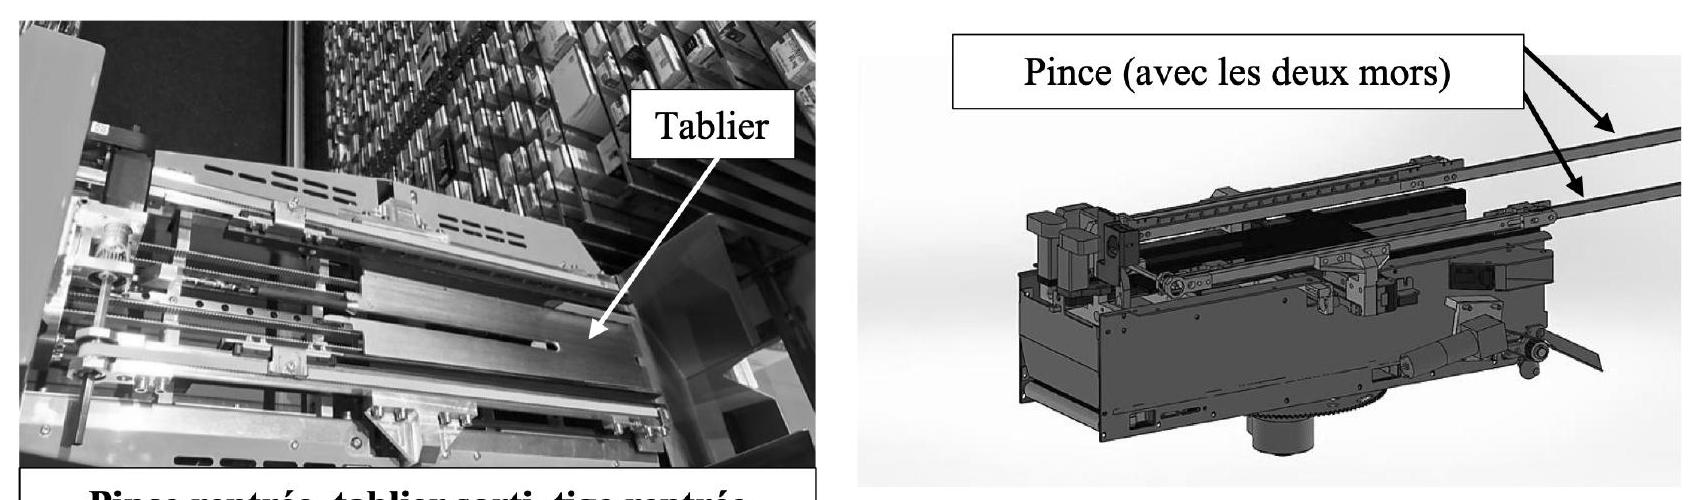
\includegraphics[max width=\textwidth, center]{fig_23_a}

Pince rentrée, tablier sorti, tige rentrée\\
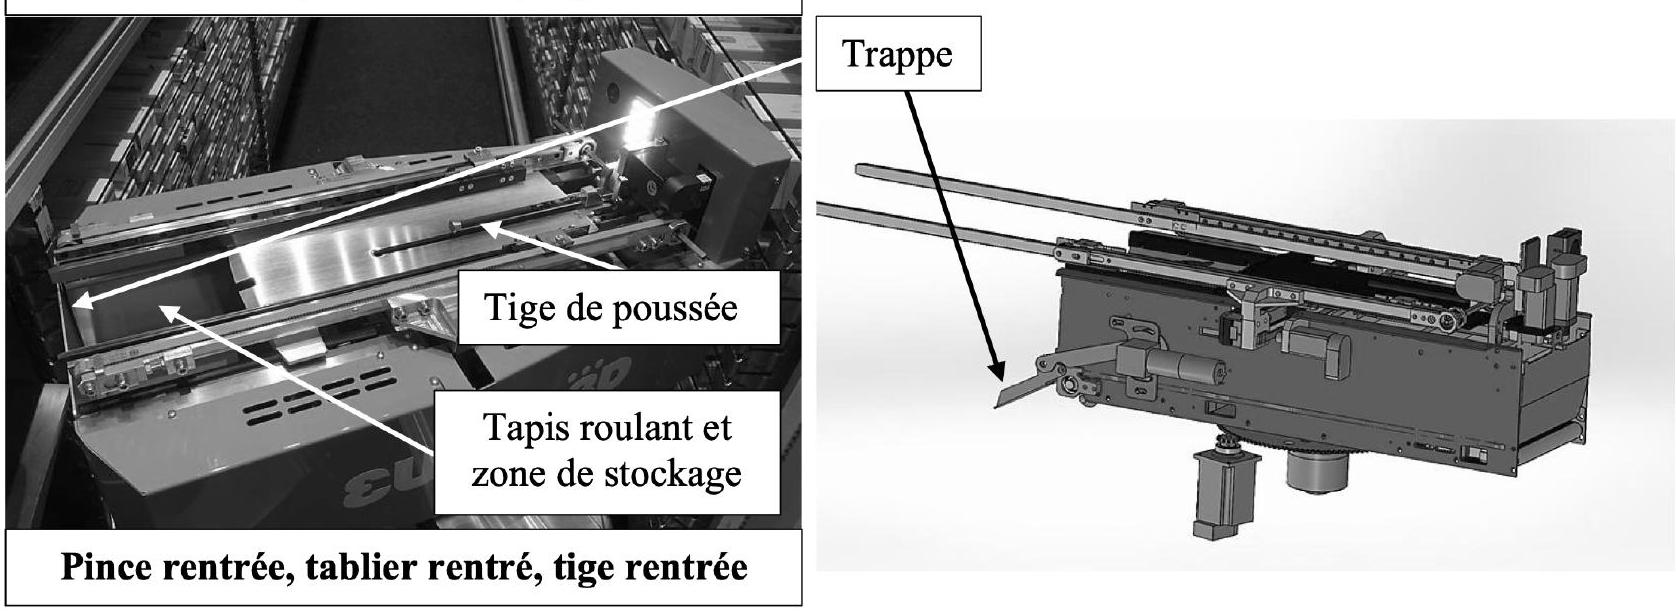
\includegraphics[max width=\textwidth, center]{fig_23_b}

\caption{\label{fig:CCS_TSI_2021_fig_23}Description de la tête EUCLID3.}
xxxxxx
\end{figure}

\begin{table}
\centering
\begin{tabular}{|c|c|c|c|c|}
\hline
\multirow{2}{*}{Sous-système} & \multicolumn{2}{|c|}{Entrées} & \multicolumn{2}{|c|}{Sorties} \\
\cline { 2 - 5 }
 & Notation & Commentaires & Notation & Durée (s) \\
\hline
\multirow{3}{*}{Translation pince} & pince rentrée &  & Sortir pince & 1,5 \\
\cline { 2 - 5 }
 & pince sortie & Sortie complète & Rentrer pince & 1 \\
\cline { 2 - 5 }
 & profondeur & \begin{tabular}{c}
Valeur de la profondeur \\
de sortie de la pince \\
\end{tabular} &  &  \\
\hline
\multirow{2}{*}{Serrage pince} & pince ouverte &  & Ecarter mors & 0,5 \\
\cline { 2 - 5 }
 & écartement & Valeur de l'écartement & Rapprocher mors & 0,5 \\
\hline
\multirow{2}{*}{Translation tige de poussée} & tige rentrée &  & Sortir tige & 2 \\
\cline { 2 - 5 }
 & tige sortie &  & Rentrer tige & 0,5 \\
\hline
\multirow{2}{*}{Translation tablier} & tablier fermé &  & Ouvrir tablier & 0,5 \\
\cline { 2 - 5 }
 & ouverture & Valeur de l'ouverture du tablier & Fermer tablier & 0,5 \\
\hline
Entraînement tapis roulant &  &  & Entraîner tapis &  \\
\hline
\multirow{2}{*}{Manouvre trappe} & trappe ouverte &  & Ouvrir trappe & 0,5 \\
\cline { 2 - 5 }
 & trappe fermée &  & Fermer trappe & 0,5 \\
\hline
\end{tabular}

\caption{\label{tab:CCS_TSI_2021_tab_06}Durées moyennes et symboles utilisés dans le graphe d'états.}
\end{table}

\begin{table}
\centering
\begin{tabular}{|l|c|c|c|c|c|c|}
\hline
Trajet & délivrance-pos1 & délivrance-pos2 & délivrance-pos3 & pos1-pos2 & pos1-pos3 & pos2-pos3 \\
\hline
Durée & 2 s & $1,4 \mathrm{~s}$ & 2 s & $1,4 \mathrm{~s}$ & 3 s & $2,5 \mathrm{~s}$ \\
\hline
\end{tabular}
\caption{\label{tab:CCS_TSI_2021_tab_07}Durées des différents déplacements.}
\end{table}

\begin{figure}
\centering
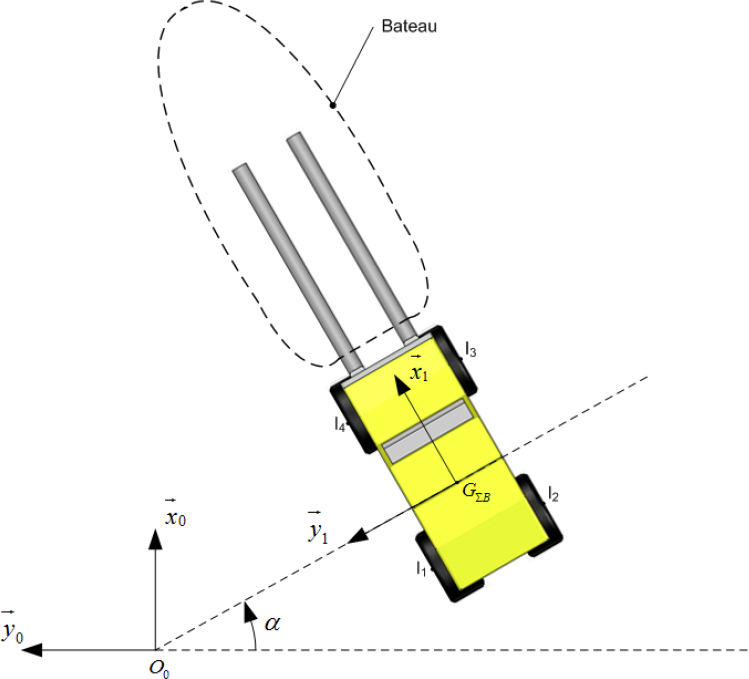
\includegraphics[max width=\textwidth]{fig_24}

\caption{\label{fig:CCS_TSI_2021_fig_24}Résultats de simulation obtenus avec la tête SLIM.}
\end{figure}

%\section*{III Validation de la structure de correction de l'axe Thêta}
\section{Validation de la structure de correction de l'axe Thêta}

\begin{obj}
Analyser l'influence du mouvement de l'axe Thêta sur les performances du système.
\end{obj}
%\section*{III.A - Analyse du mouvement de l'axe Thêta}
\subsection{Analyse du mouvement de l'axe Thêta}

\begin{obj}
Interpréter les mesures effectuées sur l'axe Thêta.
\end{obj}

Les scripts Python mis en place au début du sujet sont complétés par la prise en compte de la rotation de la tête lors d'un essai où le prélèvement s'est effectué aussi dans le magasin A. Les résultats de cet essai sont fournis à la figure \ref{fig:CCS_TSI_2021_fig_25}. Seuls les paramètres des mouvements selon X et Thêta sont donnés.

\begin{figure}
\centering
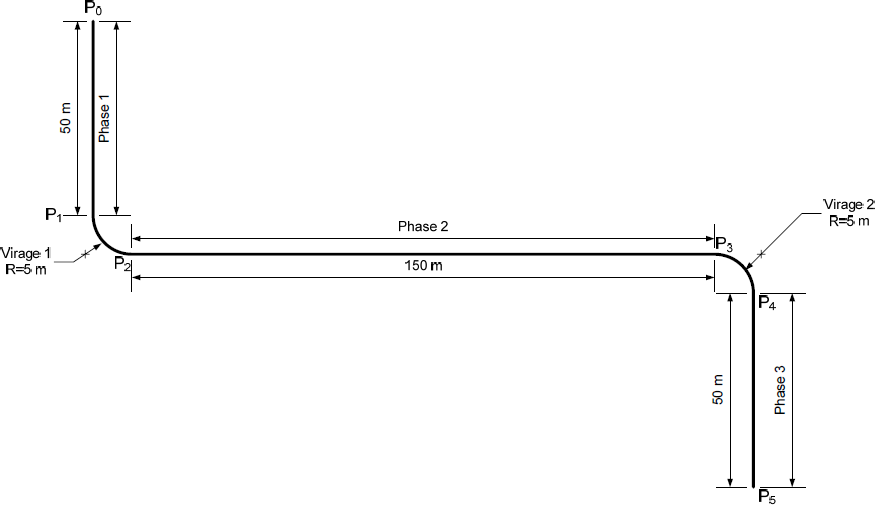
\includegraphics[max width=\textwidth]{fig_25}

\caption{\label{fig:CCS_TSI_2021_fig_25}Évolution des grandeurs cinématiques lors d'un déplacement couplé des axes (les échelles en ordonnées sont communes).}
\end{figure}

%Q 37. 
\question{Justifier l'amplitude du mouvement de l'axe Thêta et vérifier que les exigences cinématiques sont satisfaites selon cet axe.}

%\section*{III. B - Modèle causal couplé des axes X et Thêta}
\subsection{Modèle causal couplé des axes X et Thêta}
%Objectif
\begin{obj}
Mettre en évidence le couplage entre les axes X et Thêta.
\end{obj}
Dans la mesure où les mouvements sont simultanés, il existe un couplage entre les mouvements de l'axe Thêta et l'axe X.

Hypothèses: les frottements dans les liaisons et les réducteurs sont négligés, seules les actions mécaniques exercées par les moteurs et la pesanteur sont prises en compte.

Notations : $\rho_{3}=\frac{\omega(t)}{\omega_{31}(t)}=\frac{1}{10}, C_{m \theta}$ le couple moteur de l'axe Thêta, $C_{m x}$ le couple moteur de l'axe X et $M=m_{10}+m_{11}+m_{12}+m_{13}+m_{20}+m_{30}$. Les deux équations de mouvement des axes X et Thêta sont:


\begin{align*}
C_{m \theta} & =\rho_{3}\left[J_{3} \ddot{\theta}-m_{30} R_{30} \ddot{x} \cos (\theta)\right] \text { avec } J_{3}=I_{30}+m_{30} R_{30}^{2}  \tag{III.1}\\
C_{m x} & =\left(I_{11}+I_{12} \rho_{1}^{2}+M \rho_{x}^{2}\right) \dot{\omega}_{11}-\rho_{x} m_{30} R_{30}\left[\ddot{\theta} \cos (\theta)+\dot{\theta}^{2} \sin (\theta)\right] \tag{III.2}
\end{align*}


%Q 38. 
\question{À partir du schéma cinématique de la figure \ref{fig:CCS_TSI_2021_fig_A} du document réponse, énoncer le théorème utilisé (résultante ou moment en un point, appliqué à quel(s) solide(s), en projection selon quel axe) pour obtenir l'équation (III.1).}

Le schéma-bloc correspondant au couplage entre les deux axes est donné sur la figure \ref{fig:CCS_TSI_2021_fig_F} du document réponse.

%Q 39. 
\question{Compléter la zone définissant l'effet de la perturbation créée par le mouvement de l'axe X sur le mouvement de l'axe Thêta.}

Compte tenu du dimensionnement des moteurs, la perturbation de l'axe Thêta par le mouvement de l'axe X est prépondérante.

%\section*{III. $C$ - Synthèse}
\subsection{Synthèse}

Une simulation d'un déplacement couplé sur les axes X et Thêta est réalisée et fournie figure \ref{fig:CCS_TSI_2021_fig_26} avec deux valeurs différentes pour le paramètre $R_{30}$. La courbe de réponse dans le cas où $R_{30}=15 \mathrm{~cm}$ est quasiment confondue avec la courbe de consigne.

\begin{figure}
\centering
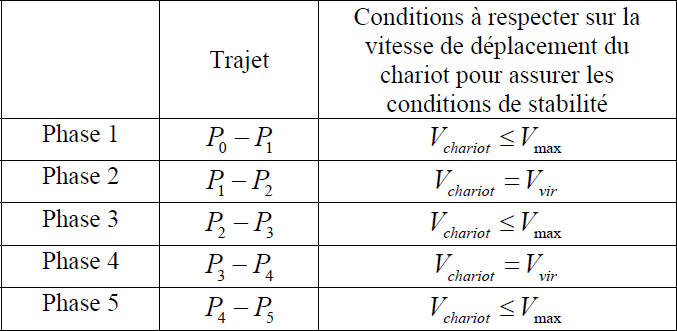
\includegraphics[max width=\textwidth]{fig_26}

\caption{\label{fig:CCS_TSI_2021_fig_26}Évolutions temporelles des déplacements de l'axe Thêta lors d'un mouvement couplé.}
\end{figure}

%Q 40. 
\question{Conclure quant à l'influence du couplage entre les deux axes sur les performances du robot Sintesi pour satisfaire les exigences de positionnement de l'axe Thêta et proposer une solution permettant de limiter la valeur de $R_{30}$ lors de la conception.}
%
%\begin{figure}
%\centering
%
\includegraphics[max width=\textwidth]{2024_07_14_db927ae3a82093776e19g-18}

